%TODO: Use LaTeX_Header
\iffalse
This file is protected by Copyright. Please refer to the COPYRIGHT file
distributed with this source distribution.

This file is part of OpenCPI <http://www.opencpi.org>

OpenCPI is free software: you can redistribute it and/or modify it under the
terms of the GNU Lesser General Public License as published by the Free Software
Foundation, either version 3 of the License, or (at your option) any later
version.

OpenCPI is distributed in the hope that it will be useful, but WITHOUT ANY
WARRANTY; without even the implied warranty of MERCHANTABILITY or FITNESS FOR A
PARTICULAR PURPOSE. See the GNU Lesser General Public License for more details.

You should have received a copy of the GNU Lesser General Public License along
with this program. If not, see <http://www.gnu.org/licenses/>.
\fi
\documentclass[10pt, a4paper, oneside]{article}

% Packages
% ---
\usepackage{ifthen}
\usepackage{enumitem}
\usepackage{float}
% not on approved list \usepackage{wrapfig}
\usepackage{helvet}
\renewcommand{\familydefault}{\sfdefault}
\usepackage{fancyhdr}
\usepackage{colortbl}
\usepackage{scrextend}
\usepackage{hyperref}
\usepackage{titlesec}
% not on approved list \usepackage[export]{adjustbox}
\titleformat{\section}{\bfseries\Large}{\thesection.}{0.5em}{}
\titleformat{\subsubsection}{}{\thesubsubsection}{1em}{\itshape}
\setlength{\parindent}{0pt}
\setcounter{secnumdepth}{0} % No numbers, but import into TOC anyway
\usepackage{textcomp} % for upquote
\usepackage{listings}
% \usepackage{wrapfig}
% \usepackage[export]{adjustbox}
% Set default for listings
\lstset{
  basicstyle=\ttfamily,
  columns=flexible,
  breaklines=true,
  breakatwhitespace=true,
  upquote=true, % Don't put weird single quotes
  % WIP: https://tex.stackexchange.com/q/385271/87531
  %  breakindent=1em,
  % literate=-{\nobreak-\nobreak}3 [--]{\nobreak--\nobreak}4, % <--- 10K penalty to break around - (e.g. python-matplotlib) https://tex.stackexchange.com/a/200498 https://tex.stackexchange.com/a/119371
}
\usepackage[margin=.75in]{geometry}
\usepackage{microtype}
\pagenumbering{roman}
\pagestyle{fancy}
\fancyhf{}
\lfoot{ANGRYVIPER IDE User Guide}
\rfoot{\thepage}
\renewcommand{\headrulewidth}{0pt}
\definecolor{blue}{rgb}{.5, .75,1}

% This block is to make sure there is 3cm min at the bottom of a page before a new section or subsection is allowed to start. Otherwise, next page.
% Modified from http://tex.stackexchange.com/a/152278
\usepackage{etoolbox}
\newskip\mfilskip
\mfilskip=0pt plus 3cm\relax
\newcommand{\mfilbreak}{\vspace{\mfilskip}\penalty -200%
\ifdim\lastskip<\mfilskip\vspace{-\lastskip}\else\vspace{-\mfilskip}\fi}
\pretocmd{\section}{\mfilbreak}{}{}
\usepackage{graphicx} % Add pictures to your document
% end [sub]section pushes
\usepackage{tabularx}
% These define tabularx columns "C" and "R" to match "X" but center/right aligned
\newcolumntype{C}{>{\centering\arraybackslash}X}
\newcolumntype{R}{>{\raggedleft\arraybackslash}X}

% \parindent=20pt
% \hangindent=0.7cm

% \tableofcontents
% \vspace{1pc}
% \hrule
\usepackage{amsmath} % Advanced math typesetting
\usepackage[utf8]{inputenc} % Unicode support (Umlauts etc.)
\usepackage[english]{babel} % Change hyphenation rules

%\usepackage[backend=bibtex,style=verbose-trad2]{biblatex} % Use biblatex package
%\bibliography{quick} % The name of the .bib file (name without .bib)

%TODO: Why doesn't this use LaTeX_Header?
\def\snippetpath{../../av/tex/snippets}
% Usage:
% \def\snippetpath{../../../../../doc/av/tex/snippets/}
% % Usage:
% \def\snippetpath{../../../../../doc/av/tex/snippets/}
% % Usage:
% \def\snippetpath{../../../../../doc/av/tex/snippets/}
% \input{\snippetpath/includes}
% From then on, you can use "input" With no paths to get to "snippets"
% You also get all "major" snippets not part of the global LaTeX_Header
% NOTE: If not using the global LaTeX_Header, you need to
% \usepackage{ifthen} to use the \githubio macro

\hyphenation{ANGRY-VIPER} % Tell it where to hyphenate
\hyphenation{Cent-OS} % Tell it where to hyphenate
\hyphenation{install-ation} % Tell it where to hyphenate

\newcommand{\todo}[1]{\textcolor{red}{TODO: #1}\PackageWarning{TODO:}{#1}} % To do notes
\newcommand{\code}[1]{\texttt{#1}} % For inline code snippet or command line
\newcommand{\sref}[1]{Section~\ref{#1}} % To quickly reference a section

% To quickly reference a versioned PDF on github.io
% \def\ocpiversion{1.5.0}
\def\ocpiversion{1.5.0rc4} % TEMPORARY

% This gives a link to github.io document. By default, it puts the filename.
% You can optionally change the link, e.g.
% \githubio{FPGA\_Vendor\_Tools\_Installation\_Guide.pdf} vs.
% \githubio[\textit{FPGA Vendor Tools Installation Guide}]{FPGA\_Vendor\_Tools\_Installation\_Guide.pdf}
% or if you want the raw ugly URL to come out, \githubioURL{FPGA_Vendor_Tools_Installation_Guide.pdf}
\newcommand{\githubio}[2][]{% The default is for FIRST param!
\href{http://opencpi.github.io/releases/\ocpiversion/#2}{\ifthenelse{\equal{#1}{}}{\texttt{#2}}{#1}}}
\newcommand{\githubioURL}[1]{\url{http://opencpi.github.io/releases/\ocpiversion/#1}}

% Fix import paths
\makeatletter
\def\input@path{{\snippetpath/}}
\makeatother

% From then on, you can use "input" With no paths to get to "snippets"
% You also get all "major" snippets not part of the global LaTeX_Header
% NOTE: If not using the global LaTeX_Header, you need to
% \usepackage{ifthen} to use the \githubio macro

\hyphenation{ANGRY-VIPER} % Tell it where to hyphenate
\hyphenation{Cent-OS} % Tell it where to hyphenate
\hyphenation{install-ation} % Tell it where to hyphenate

\newcommand{\todo}[1]{\textcolor{red}{TODO: #1}\PackageWarning{TODO:}{#1}} % To do notes
\newcommand{\code}[1]{\texttt{#1}} % For inline code snippet or command line
\newcommand{\sref}[1]{Section~\ref{#1}} % To quickly reference a section

% To quickly reference a versioned PDF on github.io
% \def\ocpiversion{1.5.0}
\def\ocpiversion{1.5.0rc4} % TEMPORARY

% This gives a link to github.io document. By default, it puts the filename.
% You can optionally change the link, e.g.
% \githubio{FPGA\_Vendor\_Tools\_Installation\_Guide.pdf} vs.
% \githubio[\textit{FPGA Vendor Tools Installation Guide}]{FPGA\_Vendor\_Tools\_Installation\_Guide.pdf}
% or if you want the raw ugly URL to come out, \githubioURL{FPGA_Vendor_Tools_Installation_Guide.pdf}
\newcommand{\githubio}[2][]{% The default is for FIRST param!
\href{http://opencpi.github.io/releases/\ocpiversion/#2}{\ifthenelse{\equal{#1}{}}{\texttt{#2}}{#1}}}
\newcommand{\githubioURL}[1]{\url{http://opencpi.github.io/releases/\ocpiversion/#1}}

% Fix import paths
\makeatletter
\def\input@path{{\snippetpath/}}
\makeatother

% From then on, you can use "input" With no paths to get to "snippets"
% You also get all "major" snippets not part of the global LaTeX_Header
% NOTE: If not using the global LaTeX_Header, you need to
% \usepackage{ifthen} to use the \githubio macro

\hyphenation{ANGRY-VIPER} % Tell it where to hyphenate
\hyphenation{Cent-OS} % Tell it where to hyphenate
\hyphenation{install-ation} % Tell it where to hyphenate

\newcommand{\todo}[1]{\textcolor{red}{TODO: #1}\PackageWarning{TODO:}{#1}} % To do notes
\newcommand{\code}[1]{\texttt{#1}} % For inline code snippet or command line
\newcommand{\sref}[1]{Section~\ref{#1}} % To quickly reference a section

% To quickly reference a versioned PDF on github.io
% \def\ocpiversion{1.5.0}
\def\ocpiversion{1.5.0rc4} % TEMPORARY

% This gives a link to github.io document. By default, it puts the filename.
% You can optionally change the link, e.g.
% \githubio{FPGA\_Vendor\_Tools\_Installation\_Guide.pdf} vs.
% \githubio[\textit{FPGA Vendor Tools Installation Guide}]{FPGA\_Vendor\_Tools\_Installation\_Guide.pdf}
% or if you want the raw ugly URL to come out, \githubioURL{FPGA_Vendor_Tools_Installation_Guide.pdf}
\newcommand{\githubio}[2][]{% The default is for FIRST param!
\href{http://opencpi.github.io/releases/\ocpiversion/#2}{\ifthenelse{\equal{#1}{}}{\texttt{#2}}{#1}}}
\newcommand{\githubioURL}[1]{\url{http://opencpi.github.io/releases/\ocpiversion/#1}}

% Fix import paths
\makeatletter
\def\input@path{{\snippetpath/}}
\makeatother


% Main document
% ---
\begin{document}
% Set up the maketitle command
\title {ANGRYVIPER IDE User Guide}
\author{}
\date{May 2019} % You can remove \today{} and type a date manually
\begin{titlepage}
\maketitle{} % Generates title
\end{titlepage}

\section{Revision History}
\renewcommand{\arraystretch}{2}
\begin{tabular}{|c|p{11cm}|c|}
\hline
Revision & Description of Change & Date\\
\hline
& Initial, from earlier doc sources & 02-2018\\ \hline
1.0 & Revision for v1.4& 09-2018\\  \hline
2.0 & Updates for v1.5 & 05-2019 \\\hline
2.1 & Converted to \LaTeX & 05-2019\\
\hline
\end{tabular}

\setcounter{tocdepth}{2}
\tableofcontents
\addcontentsline{toc}{section}{\listfigurename}
\addcontentsline{toc}{section}{\listtablename}
\newpage
\listoftables
\listoffigures
\newpage
\pagenumbering{arabic}
\section{References}
Some familiarity with the Eclipse Integrated Development Environment (IDE) or similar environment is assumed. If this is not the case, Appendix A gives basic information to get you started.

\subsection{Assumptions}
The document begins with the assumption that \href{https://github.com/opencpi/opencpi}{OpenCPI} and \href{https://github.com/opencpi/angryviper_gui}{ANGRYVIPER IDE} are installed on a development machine and the Eclipse workspace has been previously set up.
\subsection{Reference Documents}
\def\myreferences{
\hline
OpenCPI Website &
\href{https://www.opencpi.org}{www.opencpi.org} \\
\hline
OpenCPI Component Development Guide &
\githubio{OpenCPI\_Component\_Development.pdf} \\
\hline
OpenCPI Application Development Guide &
\githubio{OpenCPI\_Application\_Development.pdf} \\
}
\iffalse
This file is protected by Copyright. Please refer to the COPYRIGHT file
distributed with this source distribution.

This file is part of OpenCPI <http://www.opencpi.org>

OpenCPI is free software: you can redistribute it and/or modify it under the
terms of the GNU Lesser General Public License as published by the Free Software
Foundation, either version 3 of the License, or (at your option) any later
version.

OpenCPI is distributed in the hope that it will be useful, but WITHOUT ANY
WARRANTY; without even the implied warranty of MERCHANTABILITY or FITNESS FOR A
PARTICULAR PURPOSE. See the GNU Lesser General Public License for more details.

You should have received a copy of the GNU Lesser General Public License along
with this program. If not, see <http://www.gnu.org/licenses/>.
\fi

% This snippet creates the "References" table labeled "table:references"
% It creates three columns: Name, Publisher, Link and then inserts default documents
%
% To skip these defaults, define macros named
% refskipgs to skip "Getting Started"
% refskipig to skip "Installation Guide"
% refskipac to skip "Acronyms and Definitions"
% refskipocpiov to skip "OpenCPI Overview"
%
% See RPM_Installation_Guide.tex for examples
%
% After the defaults, it optionally inserts the "myreferences" macro that
% you defined elsewhere (you put hlines above all lines)
%
% If you want the \caption on the bottom, define "refcapbottom"
\begin{center}
\renewcommand*\footnoterule{} % Remove separator line from footnote
\renewcommand{\thempfootnote}{\arabic{mpfootnote}} % Use Arabic numbers (or can't reuse)
\begin{minipage}{0.9\textwidth}
  \begin{table}[H]
\ifx\refcapbottom\undefined
  \caption {References}
  \label{table:references}
\fi
  \begin{tabularx}{\textwidth}{|C|C|}
    \hline
    \rowcolor{blue}
    \textbf{Title} & \textbf{Link} \\
\ifx\refskipocpiov\undefined
    \hline
    OpenCPI Overview & \githubio{Overview.pdf} \\
\fi
\ifx\refskipac\undefined
    \hline
    Acronyms and Definitions & \githubio{Acronyms\_and\_Definitions.pdf} \\
\fi
\ifx\refskipgs\undefined
    \hline
    Getting Started & \githubio{Getting\_Started.pdf} \\
\fi
\ifx\refskipig\undefined
    \hline
    Installation Guide & \githubio{RPM\_Installation\_Guide.pdf} \\
\fi
\ifx\myreferences\undefined
\else
    \myreferences
\fi
    \hline
  \end{tabularx}
\ifx\refcapbottom\undefined
\else
  \caption {References}
  \label{table:references}
\fi
  \end{table}
\end{minipage}
\end{center}

\section{Introduction}
The ANGRYVIPER (AV) {IDE} consists of the Eclipse IDE for C/C++ developers and a custom plugin for OpenCPI development. OpenCPI users local to the project may install OpenCPI and the IDE from the yum repository (the IDE is a separate AV IDE RPM). Open source users must obtain the IDE plugin from GitHub and drop it into an existing Eclipse installation. Both methods are described in the \githubio[RPM Installation Guide]{RPM\_Installation\_Guide.pdf} Section 6, addresses the RPM Installation and Appendix B addresses the plugin install. Note, if the RPM method is used, the IDE is installed in \textbf{opt/opencpi/gui} and the command \textbf{ocpigui} is provided to start the IDE.
\subsection{New Features in the 1.5 Release}
In the 1.5 release, the ANGRYVIPER team focused on getting the OpenCPI XML editors current with OpenCPI Framework standards. Every available component editor (excluding the Application and Assembly Editors) is updated. In addition, new editors are provided for the Properties File, Signals File, and Slot Signals File. These editors are not integrated with the OpenCPI Projects view but they will open if the respective XML file is selected via the Eclipse Project Explorer.

\newpage
\section{Overview}
The face of the ANGRYVIPER {AV} IDE is now the \textbf{ANGRYVIPER (AV) Perspective}. This section provides an overview of the perspective layout and how to set it up in a new IDE installation.
\subsection{AV Perspective Views}
The figure below illustrates the new AV Perspective. It consists of detailed views and the Eclipse Editor panel.

\begin{figure}[h!]
	\centering
	\caption{ANGRYVIPER Perspective Views}\label{fig:AVPerspectiveViews}
	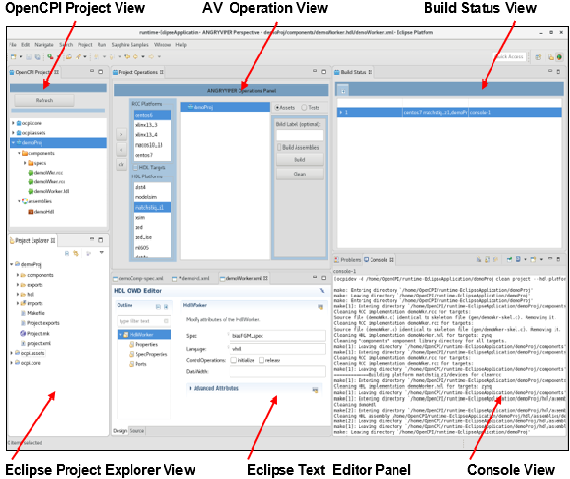
\includegraphics[width=.95\linewidth]{AVPerspectiveViews.png}
\end{figure}

Below are brief summaries of each of the perspective views, full descriptions are provided in the later sections.
\begin{itemize}
\item []	\hyperlink{OpenCPI Projects View Features}{\textbf{OpenCPI Projects View}} – an explorer giving a flattened view of the projects and assets. In the 1.4 release this view has become the primary tool to find and open asset XML files and its context menu has a rich set of features: asset wizard, open, build, clean, delete, and project registration. To open the menu simply right-click anywhere in this view.
\item [] \hyperlink{Operations View }{\textbf{AV Operations View}}– provides platform selection and controls to build assets and run tests. The AV Operations View layout has changed to provide a full feature application unit testing capability in addition to building and cleaning assets.
\item []	\hyperlink{Build Status View Features}{\textbf{Build Status View}} – provides a graphical view of build/run execution configurations and execution status. A run configuration gets a color coded status bar that visually relates status. The status bar expands to provide details and execution times of selections addressed in the run. The user can also re-run builds and tests using this view.
\item [] \hyperlink{Project Explorer View}{\textbf{Project Explorer View}} – Provides a view into a projects file system. This view primarily supports code development. It is included in the perspective for reasons provided in the Overview Section.
\item [] \hyperlink{Editor panel} {\textbf{Eclipse Editor panel}} – Asset and text editors open in this panel
\item [] \hyperlink{Eclipse Console View} {\textbf{Eclipse Console View}} – Shows the various ocpidev command executions based on user requests as well as the result of the requests.
\end{itemize}
\subsubsection{Open the AV Perspective}
 In a new Eclipse installation, the current default behavior is that Eclipse will open in the selected workspace and will display the C/C++ Perspective shown below.\\

\textbf{\emph{Note: The AV Perspective must be added to the Eclipse perspectives toolbar for regular use.}}
\begin{figure}[h!]
\centering
\caption{IDE showing C/C++ Perspective}\label{fig:IDE_CandC++Perspective}
	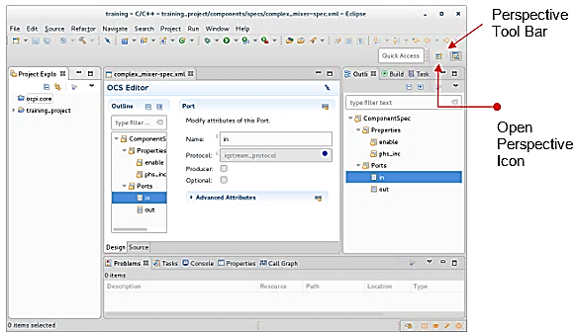
\includegraphics[width=1.0\textwidth]{CandC++.png}
\end{figure}
\subsubsection{Adding the Perspective to the Toolbar}
To open the Perspective and add it to the Perspectives Toolbar:
\begin{itemize}
\item Click the Open Perspective Icon
\item Select it from the Perspective List
\item[](Eclipse will switch to the perspective and add the AV Icon to the perspectives toolbar)
\item Click through the toolbar selections to change between perspectives\\
\begin{figure}[h!]
  \centering
  \caption{PerspectiveView}\label{fig:Perspective View}
    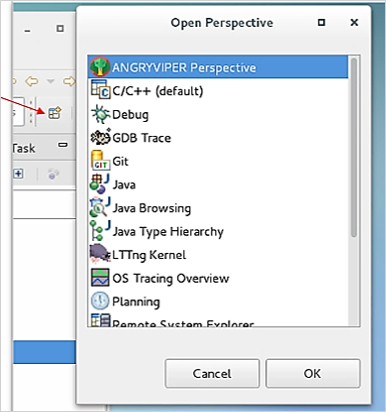
\includegraphics[width=.65\textwidth]{AVPerspectiveView.png}
\end{figure}


\textbf{\emph{Note: If the AV Perspective is not shown in this Open Perspective window, make sure the \textbf{av.proj.ide. plugin} is in your Eclipse installation}}
\item[]For personalization, Eclipse allows the user to rearrange the views in the perspective and also to add views. It will then save the rearranged perspective and will display it from this way forward, if the workspace is preserved.
\end{itemize}
To see a listing of Eclipse perspectives:
\begin{itemize}
\item Navigate to: Window
\item Navigate to: Perspective
\item Open Perspective
\item[] (A listing of views can be seen by navigating to: Window and then Show View)
\end{itemize}
\section{IDE Overview and Features}
\subsection{Overview}
The AV Perspective default layout was selected because it provides a core complement of tools to accomplish OpenCPI operations and it provides the most OpenCPI project features for the user. It is now the main display for the IDE. This section provides feature details for each of the Eclipse views that make up the perspective.
\subsection{OpenCPI Projects View Features}\hypertarget{OpenCPI Projects View Features}
The OpenCPI Projects View provides navigation into a flattened view of OpenCPI projects. It currently displays OpenCPI projects and a subset of the OpenCPI assets that it supports. A right-click context menu provides features appropriate to the selected asset.\\

\begin{figure}[h!]
\centering
   \caption{List of Features}\label{fig:ListofFeatures.png}
    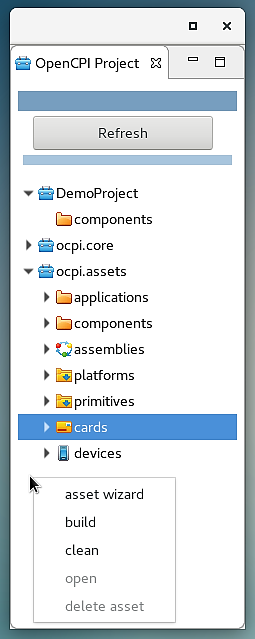
\includegraphics[width=.25\textwidth]{ListofFeatures.png}
\end{figure}
The user has the following features to choose from:
\begin{itemize}
\item	Asset Wizard – Opens the Asset Wizard
\item	Build
\item	Clean
\item	Open - When enabled, opens the assets XML file in the respective editor (double-clicking on an individual asset it will open it as well)
\item	Delete Asset – Removes the asset and its respective artifacts
\item	Build or clean can be executed from any level in the tree from entire projects to individual assets like workers and applications.
\end{itemize}

Context features are added to the menu based on the current [single] selection:
\begin{itemize}
\item	Project selected – Opens Register or Unregister depending on the registration state of the project
\item	Components selected – New Component, New Protocol, New Worker, New Unit Test
\item	Applications, assemblies, primitives Selected – Creates a new respective asset. It is also used to select assets to be added to the Operations View
\end{itemize}

\subsubsection{Building from the OpenCPI Projects View}
\begin{itemize}
\item Select one or more assets in the view and right-click
\item Select Build or Clean from the context menu
\end{itemize}
 An execution configuration is constructed from the selections, the platform selections and other inputs from the Operations panel
 The figure below displays a launch from the OpenCPI Projects View and the Status Bar for the build
\begin{figure}[h!]
	\caption{Projects View}\label{fig:ProjectsView}
	\centering
	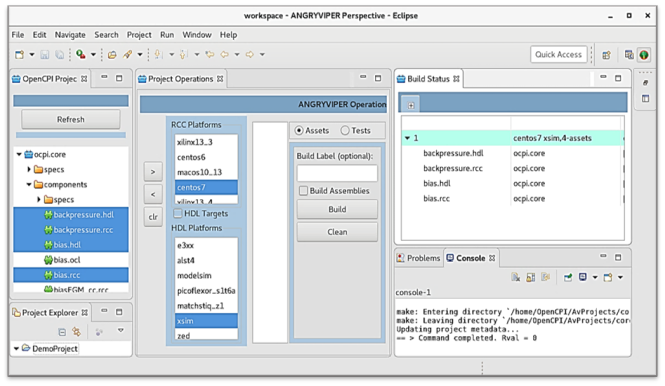
\includegraphics[width=.95\textwidth]{ProjectsView.png}
\end{figure}
\section{Operations View Features}\hypertarget{Operations View Features}
The Operations View is used to build OpenCPI assets and to
build and run application component unit tests\\

This panel has two modes of operation: \begin{enumerate}
\item Assets Mode- supports assets build and clean operations
\item Test Mode- supports unit test operations
\end{enumerate}
Core features of the panel are:
\begin{itemize}
\item Add  selections in the Projects View to the Operations panel ($>$ button)
\item Remove selected assets from the panel ($<$ button)
\item Clear the panel (clr button)
\item Make RCC/HDL platform build selections or HDL target selections
\item Execute build or clean on the assets in the Operations panel in the order they appear
\item Build and run unit tests
\end{itemize}
To add assets to the Operations Panel:
\begin{itemize}
\item Select one or more assets in the Projects panel (use the CTRL or SHIFT keys similarly to working with an email app)
\item Press the add button
\item Select the platforms for the build
\item[] The radio buttons on the top of the Build Controls section toggle controls for building assets and running unit tests.
\end{itemize}

\subsubsection{Assets Mode}
A build or clean execution is initiated by the Build/Clean buttons. Once it is initiated, an execution configuration is established. The user may repeat a build or clean execution on this configuration  from this panel or the Status Monitor View.\\

The figure below demonstrates a build executed from the Operations panel. A status bar for the completed build is expanded to show the build order. The console view lists each ocpidev build command and output from the command.\\

If the execution configuration is rerun, the corresponding status bar and console will show the progress of the execution. Building assets can occur at all levels of an OpenCPI project:
\begin{itemize}
\item Project
\item Second-Level Asset folders
\item Individual Assets
\end{itemize}

\begin{figure}[h!]
    \centering
    \caption{Build configuration setup in the Operations panel}

    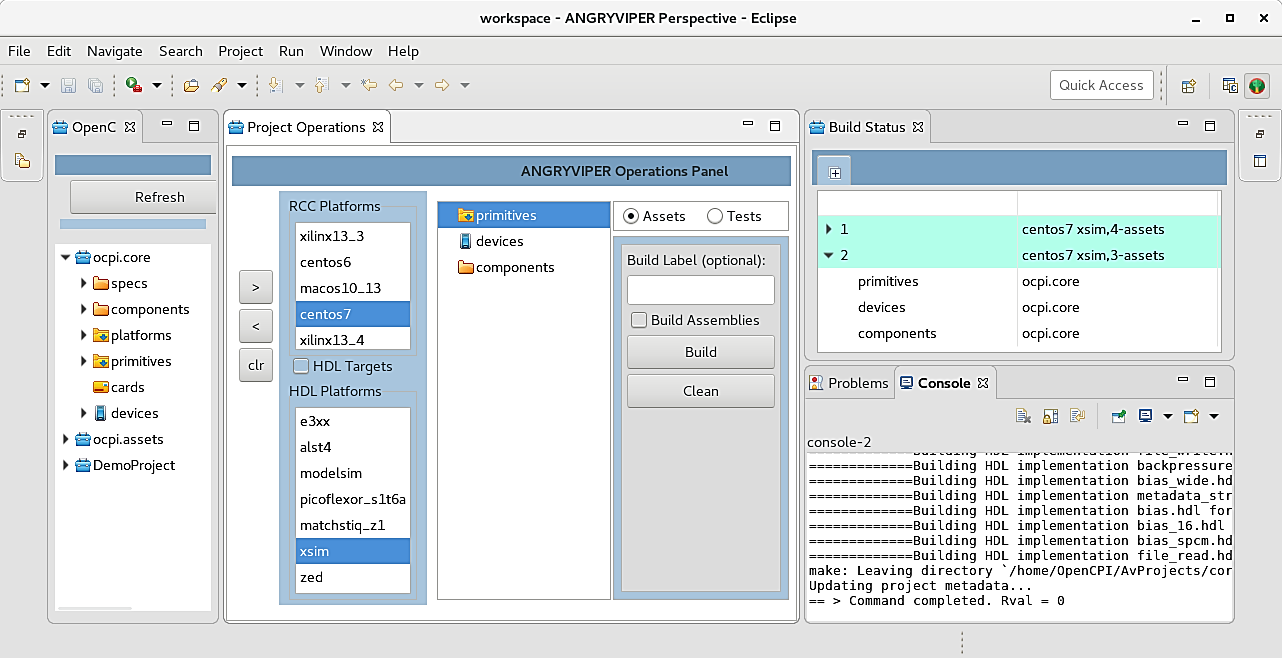
\includegraphics[width=.95\textwidth]{BuildConfigurationSetup.png}
     \label{fig:Operations panel}
\end{figure}
\subsubsection{Unit Test panel}
The Unit Tests Panel (shown in the below figure) supports most of the features for the unit testing of workers which is described in the OpenCPI \githubio[Component Development Guide]{OpenCPI\_Component\_Development.pdf}.
Reference the Component Development Guide for a complete description of the unit test of workers and details of the five phases of unit testing. The five phases of unit testing are:
\begin{enumerate}
\item Generate
\item Build
\item Prepare
\item Run
\item Verify
\end{enumerate}
The tests panel provides control for these 5 phases, \emph{(currently, there is no discrete support for the Build Phase)} and it provides three buttons that combine unit test phases that typically support development and debugging of a unit test.
\begin{figure}[h!]
    \centering
    \caption{Unit Test Panel}
    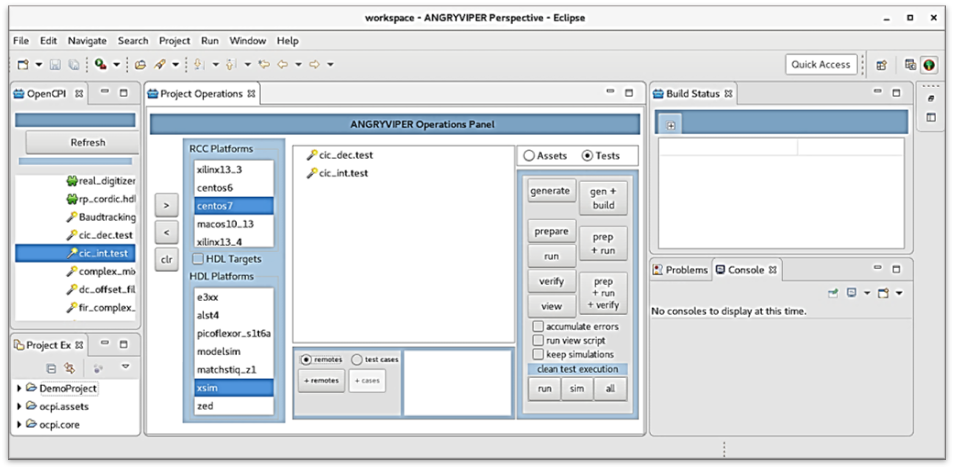
\includegraphics[width=.95\textwidth]{UnitTestsPanel.png}
      \label{fig:Unit Test panel}
\end{figure}

\subsubsection{Unit Test Features}
The following is a list of test features and the equivalent development guide operation or argument:
\begin{itemize}
\item	View Button = View Operation
\item	Run View Script = View =1
\item	Accumulate Errors = Test Accumulate Errors =1
\item	Keep Simulations = KeepSimulations =1
\item	Test Cases = Cases
\item	Remotes = OCPI\_REMOTE\_TEST\_SYSTEMS
\end{itemize}

The content of a unit test is provided in the form of: \emph{run} content, \emph{sim} (simulations data) or \emph{all} (gen/ and run/). Use the buttons in the clean test execution section to remove this content. \\

\textbf{Caution! \emph{Simulation directories may become quite large and consume an alarming amount of storage}}.\\

Similar to the Assets Mode, the Unit Test Mode constructs and executes \emph{ocpidev} command strings to perform the various phases of unit testing.\\

Building of the unit tests is possible via the Assets or Tests panel. However only the Test panel supports the other phases of unit test. Any test listed in the Operations panel is executed in sequence. \\

Prior to execution of a test phase, the user must have selected desired RCC/HDL platforms, test cases and remotes. Multiple platforms, test cases and remotes may be highlighted, but only one project for a remote system can be active.
For example:
\begin{itemize}
\item\begin{verbatim}Valid :192.168.2.9=root=root=/mnt/ocpi_core:192.168.2.10=root=root=/mnt/ocpi_assets\end{verbatim}
\item	\begin{verbatim}Invalid :192.168.2.9=root=root=/mnt/ocpi_core:192.168.2.9=root=root=/mnt/ocpi_assets\end{verbatim}
\end{itemize}
The bottom panel is used to enter remote systems and test cases. The remote/test cases radio button toggles the two operations. Click the Remotes button to add a remote system via a pop-up dialog. \\

In the example below, two remotes are available; the remote selected is placed in the next run. Test cases are added and selected in the same manner. Multiple entries may be selected for a run. The list panel has a right-click menu with edit and delete options for selected entries.
\begin{figure}[h!]
    \centering
   \caption{List panel with 2 Different Remotes}
    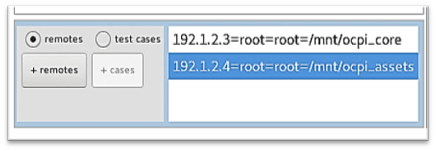
\includegraphics[width=.95\textwidth]{ListPanelwithRemotes.png}
    \label{fig:List panel with 2 Different Remotes}
\end{figure}
\subsection{Build Status View Features}
Each execution configuration has a corresponding status bar in the Build Status View. The color of the bar represents the build status:
\begin{itemize}
\item White- Indicates an active execution
\item Green- Indicates a successful completion
\item Red- Indicates a failure
\item Yellow- Indicates an execution stopped by the user
\end{itemize}
\begin{figure}[h!]
    \centering
    \caption{Build Status View}
    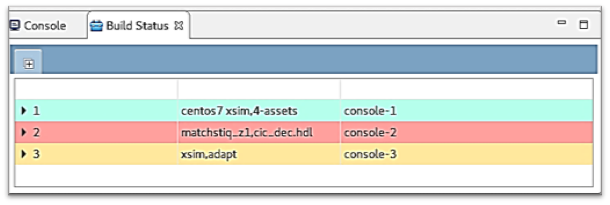
\includegraphics[width=.95\textwidth]{BuildStatusViewFeatures.png}
      \label{fig:Build Status View}
\end{figure}
The Status Bar expands to provide details about the execution and the sequence in which they occurred. In an active execution this list is dynamic; rows are added as the execution proceeds.The figure below demonstrates the Status Bar for a build that has completed successfully and the expanded view.
\begin{figure}[h!]
    \centering
    \caption{Successful Build Execution}
    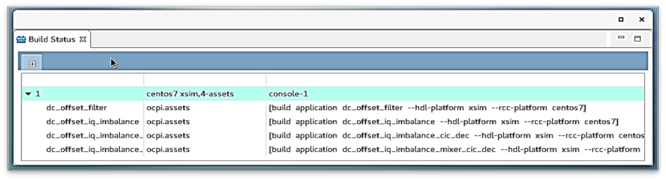
\includegraphics[width=.95\textwidth]{SuccessfulBuildExecution.png}
    \label{fig:Expanded View of Successful Build Execution}
\end{figure}

By using right-click on the status bar, several actions can be selected: \textbf{Build, Clean, Run, Stop, Delete}.\\ As an example: an inactive build execution can be rerun as a build or a clean.\\

Similarly, the user may \textbf{stop} an active execution. Finally, an inactive status bar can be deleted and when selecting a build status bar, the console for that build is brought into view.\\
\begin{figure}[h!]
    \centering
   	 \caption{Status Bar}
   		 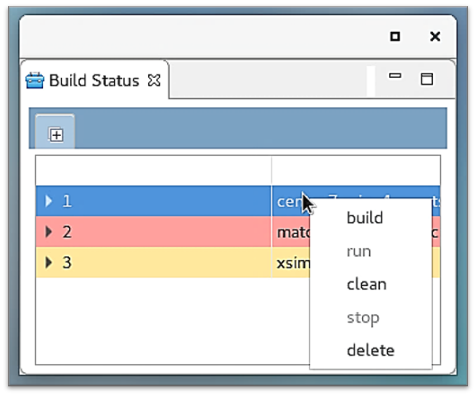
\includegraphics[width=.75\textwidth]{StatusBar.png}
     \label{fig:statusbar}
\end{figure}
\subsection{Eclipse Project Explorer View}\hypertarget{Project Explorer View}
The Eclipse Project Explorer is provided in the Perspective because it provides a \emph{file system view} of the projects. A right-click context menu provides features that are appropriate to the selected asset. \\

The user has the following features to choose from:\\

This view has a right-click context menu that provides workspace features such as:
\begin{itemize}
\item \textbf{Project Import}
\item \textbf{Workspace/Project Refresh}
\item \textbf{Access to the Assets Wizard (via the New Selection)}
\end{itemize}
It is the view Eclipse provides in the C/C++ Perspective and it is best suited to support code development.\\ However, it can be used to open OpenCPI XML files in an XML Editor and it can open supported assets in the respective graphical editor.\\

Unfortunately, it is the only view that currently supports drag and drop into the Application and Assembly Editors. Most of the core OpenCPI asset management features are now implemented in the OpenCPI Projects View.\\

\textbf{\emph{Caution! Do not delete OpenCPI assets by deleting their top-level folders in this view.}}\\

Use the \textbf{Asset Delete} provided in the OpenCPI Projects View - it executes the underlying ocpidev delete command that completely removes the asset from the framework infrastructure.\\
\begin{figure}[h!]
\centering
		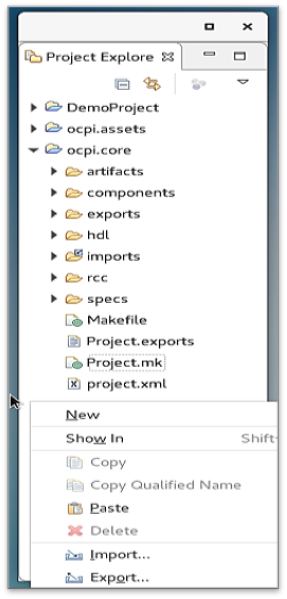
\includegraphics[width=0.35\textwidth]{EclipseProjectExplorerView.png}
	\caption{Eclipse Project Explorer View}
\end{figure}

\subsection{Eclipse Console View}\hypertarget{Eclipse Console View}
The IDE leverages the Eclipse Console View to allow the user to readily see execution output for multiple build and test runs. The IDE supports a notice console and up to fifty execution consoles.\\

There are useful features in the view toolbar: \textbf{Clear, Scroll Lock, Display Selected Console}.\\

\textbf{\emph{Note: Execution configurations will clear the respective console and bring them into view when they are rerun.}}\\

 \begin{figure}[h!]
    \centering
   	 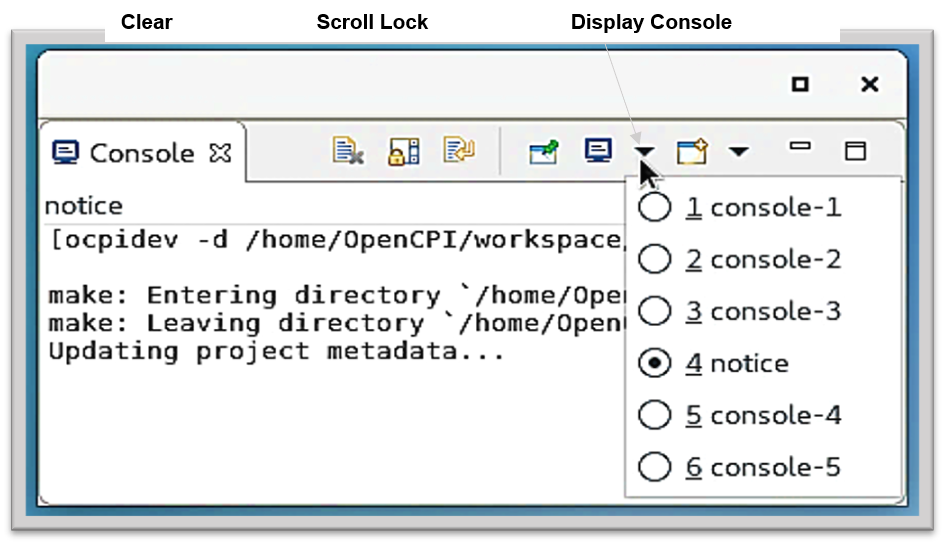
\includegraphics[width=.95\textwidth]{EclipseConsoleView.png}
     \caption{Eclipse Console View}
\end{figure}

\subsubsection{Notice Console}
\begin{itemize}
\item [] The \textbf{Notice Console} is used to communicate messages typically seen in a log. These are messages about issues in reading the environment, output of ocpidev create, delete messages, and resource issues.
\item [] View the Notice Console for notices if something unexpected happens and the IDE does not indicate a problem via a pop-up dialog.
\end{itemize}
\begin{figure}[h!]
    \centering
   	 \caption{Notice Console View}
   		 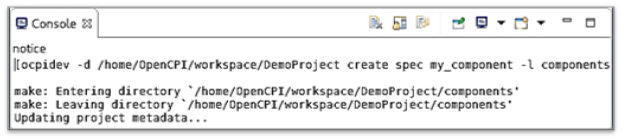
\includegraphics[width=\textwidth]{Noticeconsole.png}
\end{figure}

\subsubsection{Execution Consoles}
Execution consoles provide \textbf{build and run} commands and their output.The IDE supports up to fifty (50) active execution configurations at a time and each configuration gets its own console. The figure below shows a console for a successful build.
\begin{figure}[h!]
	\centering
	\caption{Execution Console}\label{fig:ExecutionConsole.png}
	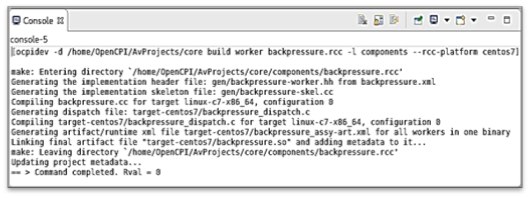
\includegraphics[width=.85\textwidth]{ExecutionConsole.png}
 \end{figure}
\subsection{OpenCPI Asset Wizard}
The \textbf{Asset Wizard} provides a tool to create a number of OpenCPI Assets. It provides a simple form for required and optional parameters to create the asset (accomplished by ocpidev create). Upon completion, the asset and follow-on OpenCPI framework folders and files will be created. \\

The new asset is displayed in the project views. If an XML Editor is provided in the IDE, then the respective Editor is opened to further populate the XML specification. The figure below shows all of the available assets in the drop-down list that the wizard supports.
\begin{figure}[h!]
	\centering
	\caption{Asset Creation Wizard}\label{fig:AssetCreationWizard}
	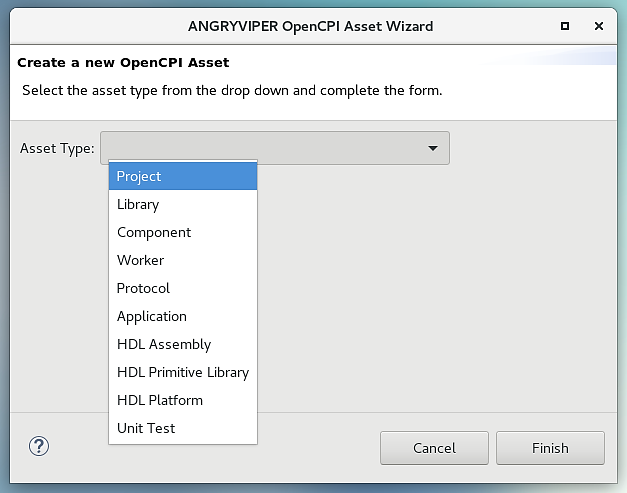
\includegraphics[width=.85\textwidth]{AssetCreationWizard.png}
 \end{figure}
This OpenCPI \textbf{Asset Creation Wizard} may be selected from the context menu obtained by right-clicking anywhere in OpenCPI Projects View.\\

It is also found under the New selection (or New Other) Eclipse Project Explorer View context menu or under the File Tab in the top Eclipse menu bar.\\

\textbf{\emph{Caution! There are some dependencies to create assets. An OpenCPI project must be open in the workspace before any other assets can be created. Also, a components library must be established before components and workers can be created}}.

\subsection{OpenCPI Asset XML Editors}
The IDE supports the creation of the following OpenCPI Assets and provides graphical editors to populate their XML files:
\begin{itemize}
\item \textbf{Component Spec} – OCS Editor
\item \textbf{Protocol Spec} – OPS Editor
\item \textbf{Component Properties File} – Properties File Editor
\item \textbf{RCC Application Worker} – OWD RCC Editor
\item \textbf{HDL Application Worker}– OWD HDL Editor
\item \textbf{HDL Assembly} – OHAD Editor
\item \textbf{HDL Signals File} – Signals File Editor
\item \textbf{HDL Slot File} – Slot File Editor
\item \textbf{OpenCPI Application} – OAS Editor
\item \textbf{HDL Platform Worker} – HDL Platform Editor
\item \textbf{Component Unit Tests} – Unit Test Editor
\end{itemize}
There are two implementations of the XML editors in the plugin. The \textbf{Component} editors are \emph{form-based} while the \textbf{Application and Assembly} editors are \emph{diagram-based} and support the form-based feature.
\subsubsection{Form Based Graphical Editors}
The Graphical Editor has two panels:
\begin{enumerate}
\item \textbf{Outline} panel
\item \textbf{Form-Input} panel
\end{enumerate}
In the example below, the Outline Panel is used to navigate the XML elements for this worker. These are the Top-Level HdlWorker Elements and Property, SpecProperty and Port (StreamInterface) child elements. Select the element in the outline to add a new one or select an existing one to see or and modify it.
\begin{figure}[h!]
	\centering
	\caption{Modify Attributes of HDL Worker}\label{fig:ModifyAttributesofHDLWorker}
	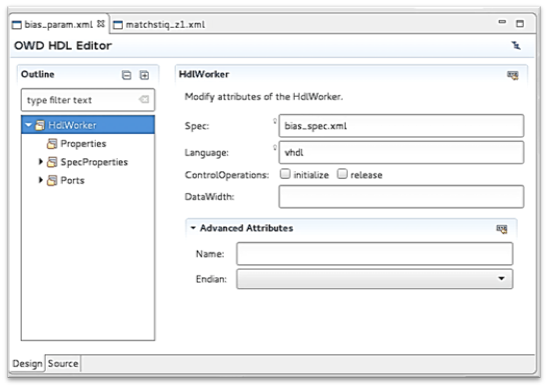
\includegraphics[width=.95\textwidth]{ModifyAttribHDLWrkr.png}
 \end{figure}
The figure below is an example of adding a property element to the worker.
Select the Properties element in the outline, then Right Click and Add Property.
\begin{figure}[h!]
	\centering
	\caption{Add a Property to a Worker}\label{fig:AddaPropertyWorker}
	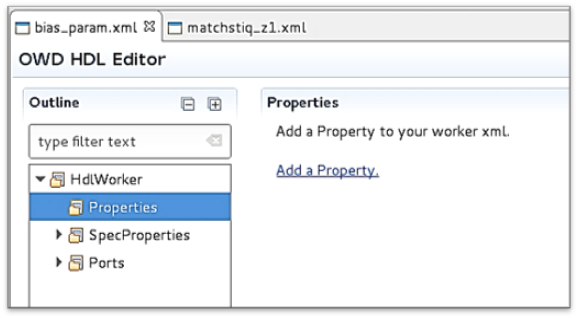
\includegraphics[width=.95\textwidth]{AddaPropertyWorker.png}
 \end{figure}
The form to populate the new element appears as shown in the Form Input panel image below.\\
\begin{figure}[h!]
	\centering
	\caption{HDL Property Element Form}\label{fig:HDLPropertyElementForm}
	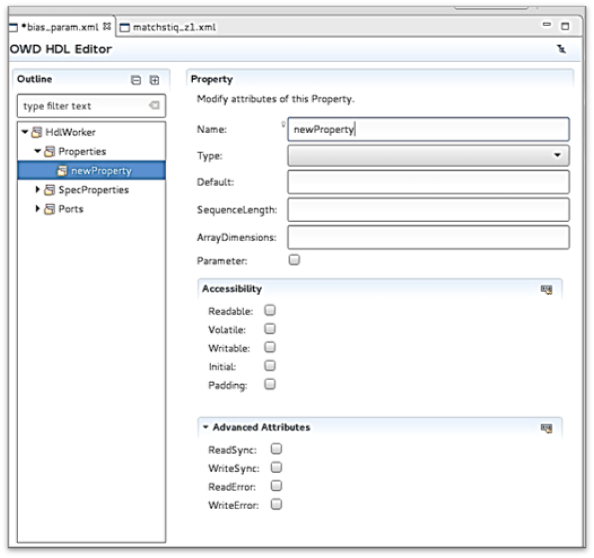
\includegraphics[width=.95\textwidth]{HDLPropertyElementForm.png}
 \end{figure}

Select the Source Tab to see how the new element is added to the XML file. \\
To remove an element:
\begin{itemize}
\item Select
\item Right Click
\item Select Delete
\end{itemize}
The source file may also be edited and those changes will appear in the design view.\\

See the \githubio[Component Development Guide]{OpenCPI\_Component\_Development.pdf} for more information about the XML files these editors support. \\

\textbf{\emph{Note: In Release 1.5 these editors were updated to current OpenCPI standards}}.\\

\subsubsection{Graphical Drag-and-Drop Editors}
The Application and Assembly Editors provide a \textbf{diagram interface} to generate the respective XML files.
\begin{figure}[h!]
	\centering
	\caption{Graphical Drag and Drop Editors}\label{fig:GraphicalDragandDropEditors}
	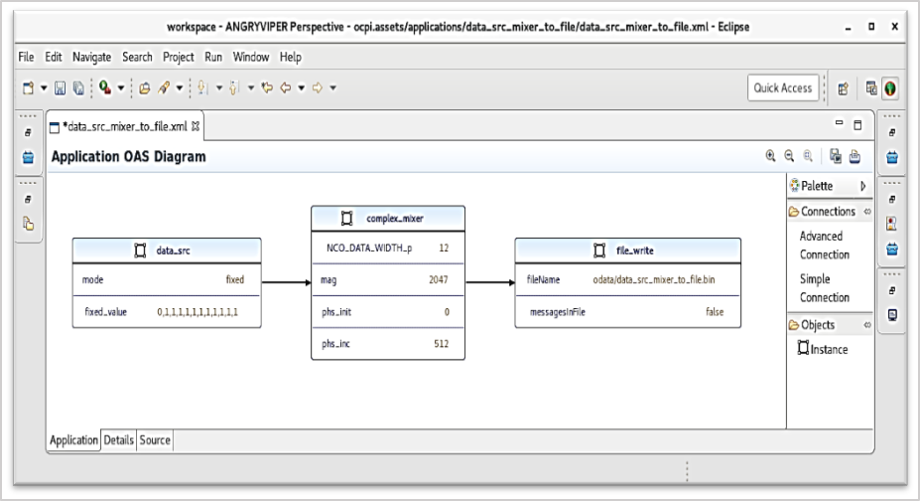
\includegraphics[width=\textwidth]{GraphicalDragandDropEditors.png}
 \end{figure}

\subsubsection{Asset XML Examples}
The following list provides OpenCPI asset XML to examine in its respective Editor. Use the OpenCPI Projects View to navigate into the OpenCPI Core and Assets projects and open the various asset XML files by doubling-clicking the asset. \\
\begin{enumerate}
\item	\textbf{OPS Editor-} core-specs-iqstream\_protocol.xml
\item	\textbf{OCS Editor-} core-components-specs-bias\_spec.xml
\item	\textbf{OWD RCC Editor-} core-components-bias\_cc.rcc
\item	\textbf{OWD HDL Editor-} core-components-bias\_param.hdl
\item	\textbf{HDL Assemble Editor-} assets-assemblies-cic\_int\_dc\_offset\_iq\_imbalance\_mixer\_cic\_dec
\item	\textbf{OAS Editor-} assets-applications-data\_src\_mixer\_to\_file
\item	\textbf{Platform Worker Editor-} assets-platforms- matchstiq\_z1
\item	\textbf{Unit Test Editor-} core-components-metadata\_stressor.test
\end{enumerate}

\subsubsection{Additional Notes About the Perspective}
The ANGRYVIPER Team hopes to continue to add capabilities to the \emph{OpenCPI Projects View} to further support OpenCPI operations. The goal for Version 1.4 was to give complementary features. This section provides a brief discussion to make the user aware of a number of issues that may occur when using the IDE.
\subsection{The Execution Configuration}
The \textbf{Execution Configuration} provides a means to associate and manage resources tied to the execution. These are:
\begin{itemize}
\item	Selected Assets and Platforms
\item	Execution Number
\item	Status Bar
\item	Console
\end{itemize}
The perspective allows limitless execution configurations,  however,  it only allows so many to exist at once since they tie together Eclipse resources such as the consoles. The current limit is fifty(50). \\

When the limit is met, the user will get a pop-up dialog that instructs the user to delete some status bars to free up resources. This is the only way to free up resources other than closing and re-launching Eclipse. The Status View allows multiple delections for this reason. Once done, execution numbers will continue to increase but consoles will be reused.

\subsection{XML Editors-Modifying Existing XML Files}
The following Editors will modify existing XML files when they are opened with the Editor. The IDE will indicate this is occurring and why; however, it will only do it once per Eclipse session.\\
The Editors are:
\begin{itemize}
\item	\textbf{OAS Editor} - The Application Editor adds a name attribute to the instance element to better support presentations
\item	\textbf{HDL Platform Editor} - This Editor will update slot signal definitions to the current standard where signal name and direction are discretely stated. Also note that if signal definitions were updated by the Version 1.4 GUI, these will have an unnecessary extension tag. If present, these may be removed manually.
\item	[]The signal and slots file editors will similarly update old signal definition formats (used a direction=$<$name$>$ attribute).
\item [] The modifications do not have to be saved.\
\end{itemize}
\textbf{\emph{Note: Signal definition changes represent the current OpenCPI standard}}.
\subsection {Warning about a Non-OpenCPI Project}
The perspective obtains asset information from the top level project.xml files. If an Eclipse workspace project is encountered that does not have a project.xml file, it is assumed the project is not an OpenCPI project. This is communicated in the Notice Console. If the project is an OpenCPI project, then something is wrong in the project file structure that does not allow project.xml to be generated.
\subsection{The Perspective is Not in Sync with the Workspace or the File System}
The OpenCPI Projects View does not track changes to the Workspace or the files system. This means changes made to a project outside of the IDE will not be apparent in the project explorers nor seen in current asset lists within the IDE. This means assets created or removed via command line will not be presented in either the Eclipse Project Explorer or OpenCPI Projects Views until both views are refreshed. Refresh the Eclipse Project view first then the OpenCPI Projects View.\\

\textbf{\emph{Note: Do not delete a project using Project Explorer or Shell Command. Use the ocpidev command to delete a project. This will ensure project registration information remains up to date.}}
\section{OpenCPI Development Workflow Using the IDE}
\subsection{Introduction}
The IDE supports a number of OpenCPI workflow concepts; beginning with setting up the OpenCPI core and assets projects and getting them built to support new project development. This section demonstrates a number of the fundamentals discussed in Sections 4 and 5 of the \githubio[Getting Started Guide]{Getting\_Started.pdf}. This includes creating the DemoProject and then a number of assets that go in the project as described in the document. Additionally, the IDE provides an effective way to look at existing assets OpenCPI XML specifications.
\subsection{OpenCPI the Core and Assets Projects}
A number of existing projects are provided in OpenCPI Release for use in development. If they are to be used, they need to be set up in the development environment, registered, and imported into the IDE and built for the desired platforms to further support new development. Procedures to set these projects up:
\begin{enumerate}
\item	Select an area in the file system to put these projects and create the folder if necessary
\item	Execute the project copy script ocpi-copy-projects to load these projects in desired folder and register them in that location (this script is interactive or arguments may be supplied)
\item	Import the desired projects into Eclipse
\end{enumerate}
\begin{figure}[h!]
	\centering
	\caption{Procedures to use existing Projects}\label{fig:Procedures to use existing Projects}
	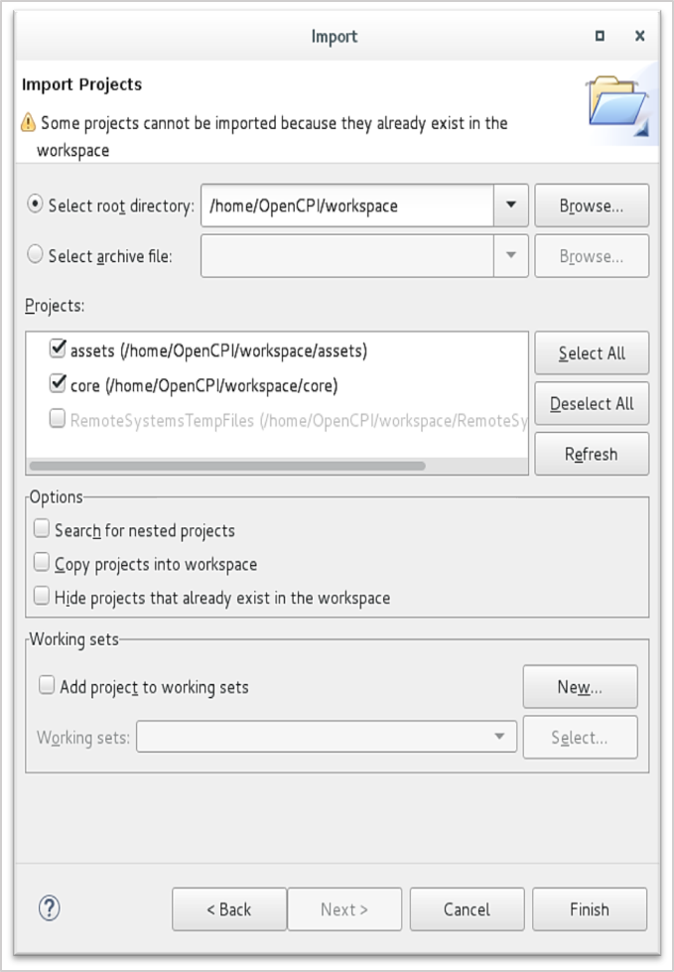
\includegraphics[width=.60\textwidth]{ProcedurestouseexistingProjects.png}
 \end{figure}
\subsection{Importing OpenCPI Core and Asset Projects}
This demonstration describes the procedure to import the core and assets projects.
\begin {enumerate}
\item	Place the cursor in the Eclipse Project Explorer panel
\item	Right Click -Import-General-Existing projects into workspace - (This opens the import wizard)
\item	Click Browse for the select root directory input
\item	Navigate to and select the folder holding these projects
\item	Select the checkboxes on the desired projects to import as shown in the preceding figure
\item	Click Finish and the projects will be brought into the Eclipse workspace - (they will appear in the Eclipse Project Explore View)
\item	Click Refresh in the OpenCPI Projects View to update that view with the imported projects
\end{enumerate}
\begin{figure}[h!]
	\centering
	\caption{Importing OpenCPI Core and Assets}\label{fig:Importing OpenCPI Core and Assets}
	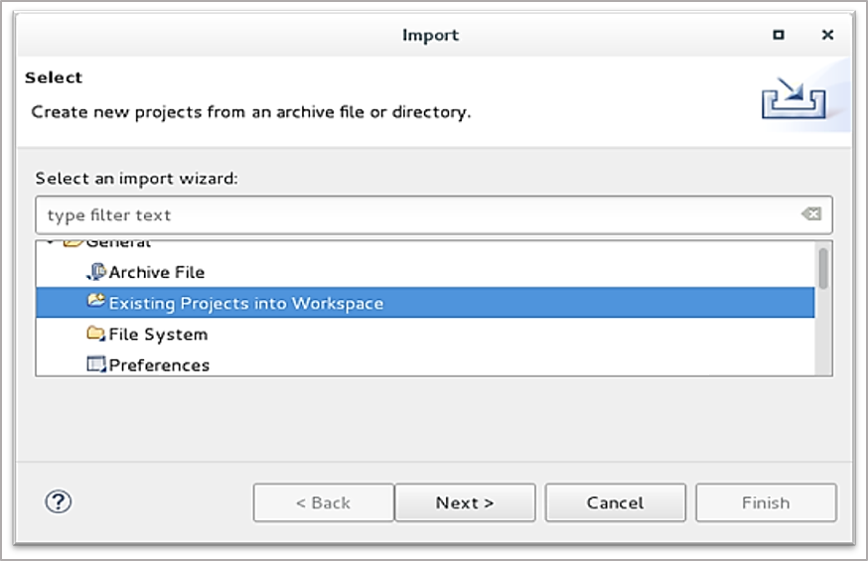
\includegraphics[width=.80\textwidth]{ImportingOpenCPICoreandAssets.png}
 \end{figure}
\subsection{Build the Projects for the desired RCC and HDL Platforms}
There are a number of ways to build existing projects in the IDE because builds can be kicked off concurrently. If time is not an issue, put the core and assets projects in the Operations panel (core first followed by assets), Select the platforms to which to build to and launch the build (press build). Core will be built followed by assets.
Concurrent building saves time-key things to know:
\begin{itemize}
\item	HDL libraries in the core project must be built before starting a build on the assets project primitives
\item	Project primitives must be built first
\item	HDL card and device libraries (cards and devices) can be built concurrently after primitives. Core components and asset primitives can be built concurrently after core HDL libraries are built
\item	Follow this sequence to build HDL libraries in the assets project
\item	Once projects components are built, it is recommended that a top-level project build is executed to ensure all build artifacts and exported properly for dependent projects
\item	Assemblies may be built concurrently
\end{itemize}
The following examples demonstrate executing builds using the IDE:
\begin{enumerate}
\item	Select the platforms for the build. In the example, RCC platform centos7 and HDL platform xsim are Selected
\item	Expand the ocpi. core project in the OpenCPI Projects View, select Primitives, right click, select Build. The build status entry appears and turns green when the build successfully completes.
\begin{figure}[h!]
	\centering
	\caption{Build Entry}\label{fig:Build Entry}
	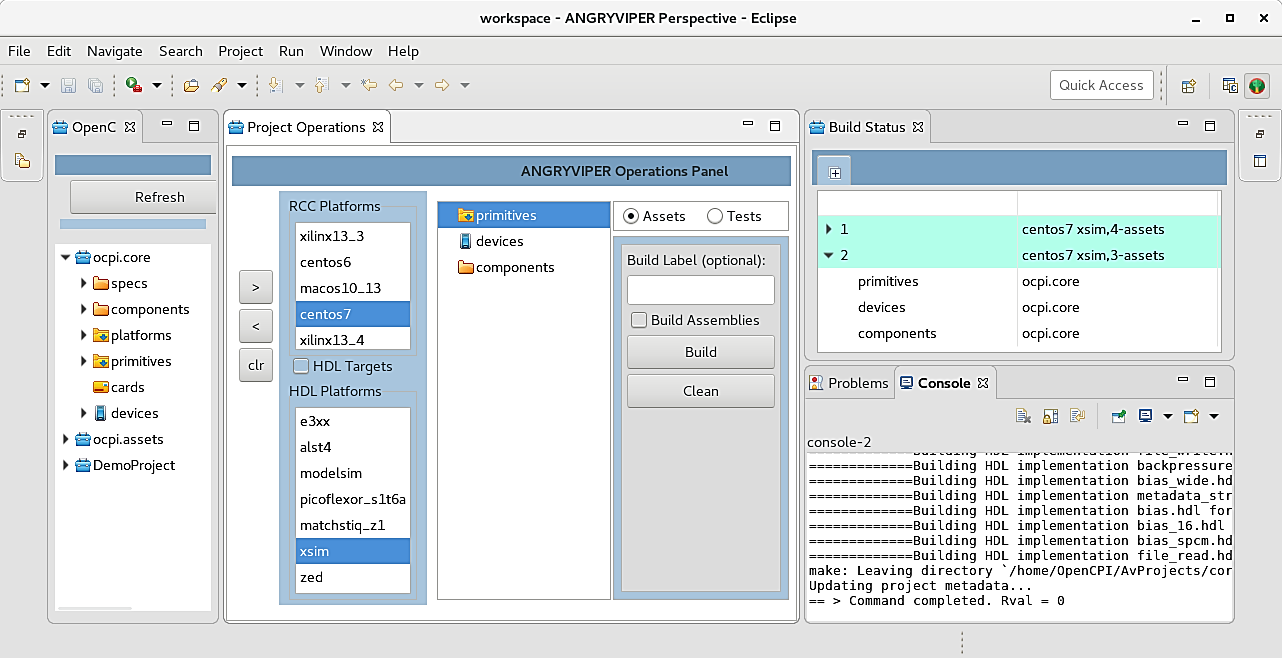
\includegraphics[width=.90\textwidth]{BuildEntry.png}
 \end{figure}

\item Select Devices (the core projects have no cards currently), right click, select Build
\item Similarly start builds for the core projects components and the assets project primitives
\begin{figure}[h!]
	\centering
	\caption{Project Built from Operations panel}\label{fig:Project Built from Ops panel}
	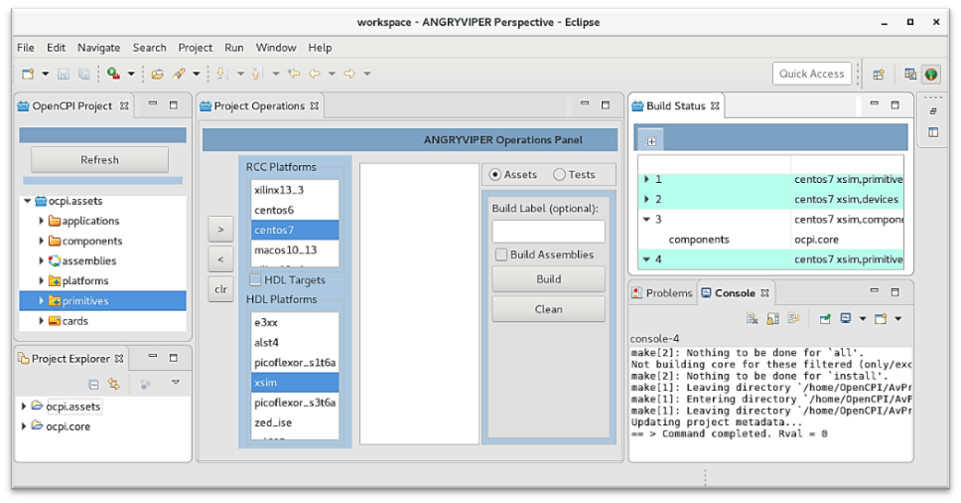
\includegraphics[width=.90\textwidth]{ProjectBuiltfromOpsPanel.png}
 \end{figure}

\item	Complete a top-level build for the core project. In this example, the core project is built from the Operations panel.
\begin{figure}[h!]
	\centering
	\caption{Core Project Built from Ops panel}\label{fig:Core Project Built from Ops panel}
	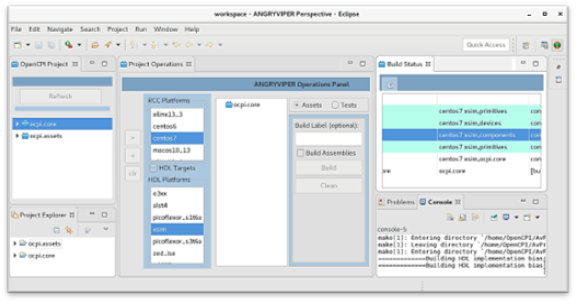
\includegraphics[width=.90\textwidth]{CoreProjectBuiltfromOpsPanel.png}
 \end{figure}

\item	Complete building the assets project following a similar process.
\end{enumerate}

\subsection{Creating New Projects and Libraries}
To create a new project:
\begin{itemize}
\item	Place the cursor in the OpenCPI Projects panel
\item	Right click
\item Select-Asset Wizard
\item	Select- Asset Type Project from the drop-down
\item	Click Finish
\end{itemize}
\textbf{\emph{Note: All registered OpenCPI projects have the core project dependency by default.}}\\

When this completes, a new project (DemoProject) will be created, registered and is displayed in the OpenCPI Projects and the Eclipse Project Explorer views. It will have the assets project as a dependency, so it can use the components contained in it. \\

\begin{figure}[h!]
	\centering
	\caption{Create a New Project}\label{fig:CreateaNewProject}
	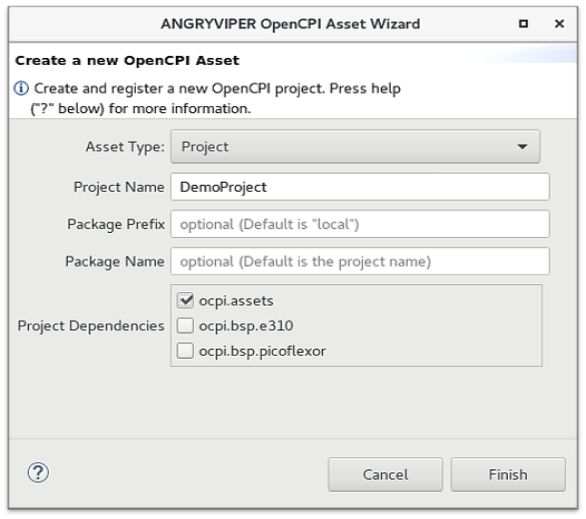
\includegraphics[width=.75\textwidth]{CreateaNewProject.png}
 \end{figure}

Next, a components library is added to DemoProject
\begin{itemize}
\item	Select the project in the OpenCPI Projects View
\item	Right Click, Open the Assets Wizard
\item	Select- Asset Type Library
\end{itemize}
The wizard will create the components library by default. If multiple libraries are anticipated, then this library should be named accordingly, and it will be placed in a top-level components folder. This example uses one components library and when complete, select Finish.

The Components Library is now created and appears in the Project Explorers as shown below:

\begin{figure}[h!]
	\centering
	\caption{Asset Wizard}\label{fig:AssetWizard2}
	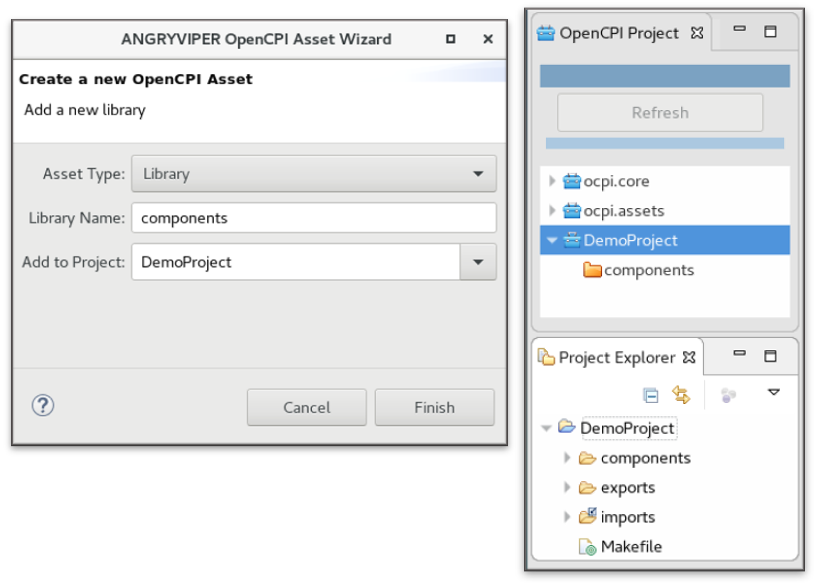
\includegraphics[width=.90\textwidth]{AssetWizard2.png}
 \end{figure}
\subsection{More on OpenCPI Projects}
In OpenCPI, package-ids are assigned to projects and other shared assets in the project, such as its libraries.\\
 The project wizard provides inputs for the project package-id: package-prefix and package-name. The project package-id is \emph{package-prefix.package-name}. This becomes a unique identifier to the project and its shared assets. The Project Wizard screen goes more into detail.\\

In the new project example above, no inputs were provided for package-prefix and package-name, the defaults are used and the assigned package-id is: local. DemoProject. This can be seen in the Project Registry.\\ To view project registry in a terminal window, \textbf{use the command: ocpidev show registry} and the result is shown below:
\begin{figure}[h!]
	\centering
	\caption{Terminal Window View}\label{fig:TerminalWindowView}
	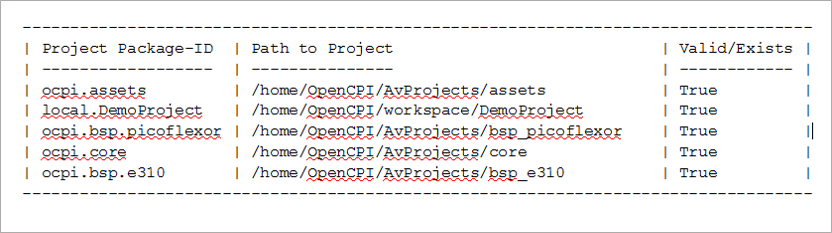
\includegraphics[width=.75\textwidth]{TerminalWindowView.png}
 \end{figure}
\subsection{Project Registration}
By registering a project, a user is publishing his/her project so that it can be referenced/searched by any user or project using that same project registry. The default project registry is found at : \textbf{ /opt/opencpi/project-registry}. The registration features are provided to support bringing in an external OpenCPI project or a project location needs to change.
Examples:
\begin{itemize}
\item	To rename a project: unregister it, and change its name with Project Explorer, refresh OpenCPI Projects, re-register it.
\item	To move a project: unregister it then delete it from the workspace (use Eclipse Project Explorer, do not delete it from the file system). Move it, import it back into the workspace, then refresh OpenCPI Projects. Now re-register it.
\end{itemize}
\subsection{Errors in Creating New Project}
If an error occurs, the wizard will present a dialog panel explaining the problem. Errors will occur when the framework cannot support the asset creation or there are file system issues. \\

Click OK to close the dialog. If the framework fails to create an asset it automatically cleans remnant artifacts off the file system.
\subsection{OpenCPI Libraries}
An OpenCPI project can have one or more libraries. The typical guidelines are as follows:
\begin{itemize}
\item A project anticipated to have a single component library, name the library components. All component and worker assets will reside in the top-level components directory. When using the OpenCPI asset wizard to create a library the default name provided is components
\item A Project anticipated to have multiple libraries, give these libraries a name other than components. These libraries will be placed in top-level components as sub-directories named after the library. The user will be given the option to create component specifications and workers in these sub-directory libraries
\item Once an option is Selected it cannot be changed without a lot manipulation
\end{itemize}
\subsection{Creating Components, Protocols and Workers}
Some fundamentals regarding creating components, protocols, and workers:
\begin{itemize}
\item Protocols specify expected data for component ports
\item Protocols and components can exist in in either the top-level specs folder of the project or in a library specs folder
\item The top-level specs folder is intended to hold more global protocols and components that can be reused in library component specifications
\item Workers may only reside in a library
\end{itemize}
The IDE’s Asset Wizard provides an easy way to create this class of assets and locate them in their proper place. Protocols and components simply need a name and where to put them. Workers need a name, component specification, and the implementation language.
\subsection{Component Example from the Getting Started Guide}
In this example, the ramp component is created using the IDE.
\begin{itemize}
\item Open the Asset Wizard
\item OpenCPI Projects
\item Select DemoProject/Components and right-click
\item Select Component from the context menu
\item Fill in the name as shown below
\end{itemize}
\begin{figure}[h!]
	\centering
	\caption{Create a New OpenCPI Asset}\label{fig:CreateaNewOpenCPIAsset}
	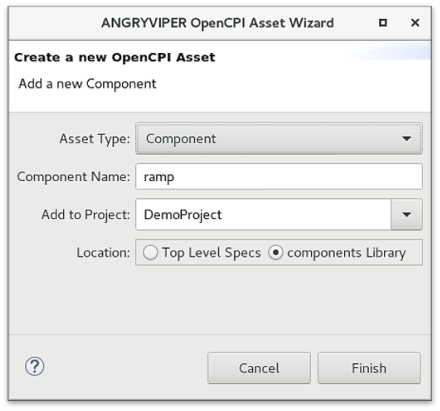
\includegraphics[width=.65\textwidth]{AssetWizard.png}
 \end{figure}
\begin{itemize}
\item Once the OCS Editor opens, select Ports in the outline
\item Click the Add a Port link and the Port Form appears and name the Port \textbf{in}
\item Select \textbf{restream protocol} from the drop-down menu
\item Repeat above and add the \textbf{out} port
\item The figure below shows the Port form for the ramp \textbf{in}
\end{itemize}
\begin{figure}[h!]
	\centering
	\caption{Port Form for the Ramp In}\label{fig:PortFormfortheRampIn}
	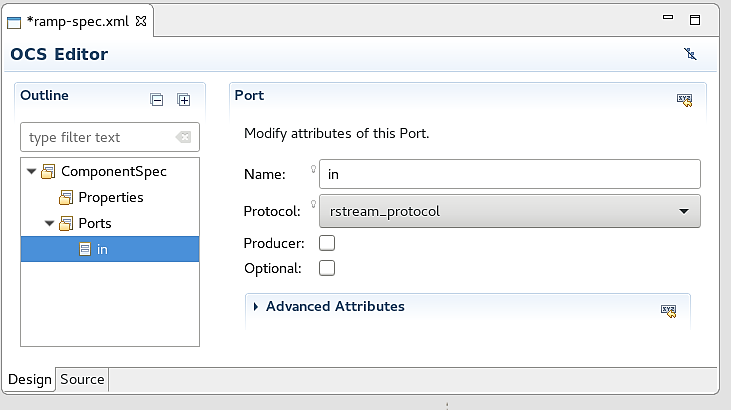
\includegraphics[width=.85\textwidth]{PortFormfortheRampIn.png}
 \end{figure}
\subsection{Worker Example from the Getting Started Guide}
\begin{itemize}
\item	Open the Asset Wizard
\item	OpenCPI Projects, Select \textbf{ramp-spec.xml} located in DemoProject/Components/specs
\item	Right-click, Select Worker from the context menu, fill in the name
\item	Select the VHDL language as shown below
\item	When the HDL OWD Editor opens, verify the spec and language entries
\item	Save both files (Eclipse floppy disks icon in the toolbar at the top)
 \end{itemize}
\begin{figure}[h!]
	\centering
	\caption{Worker Example}\label{fig:WorkerExample}
	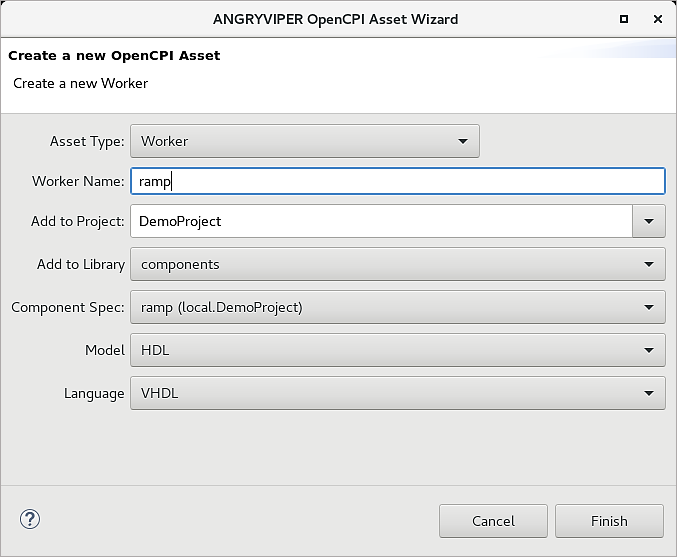
\includegraphics[width=.65\textwidth]{WorkerExample.png}
 \end{figure}
The next step is to add the \textbf{in and out} stream interfaces:
\begin{itemize}
\item	Select Ports in the HDL OWD Editor outline
\item	Click the Add a StreamInterface link and the StreamInterface form will display
\item	Set the Port name and data width as shown in the figure below
\item	As above, create the \textbf{out} Port - the ramp worker is now complete
 \end{itemize}
\begin{figure}[h!]
	\centering
	\caption{Addition of In and Out Interfaces}\label{fig:AdditionofInandOutInterfaces}
	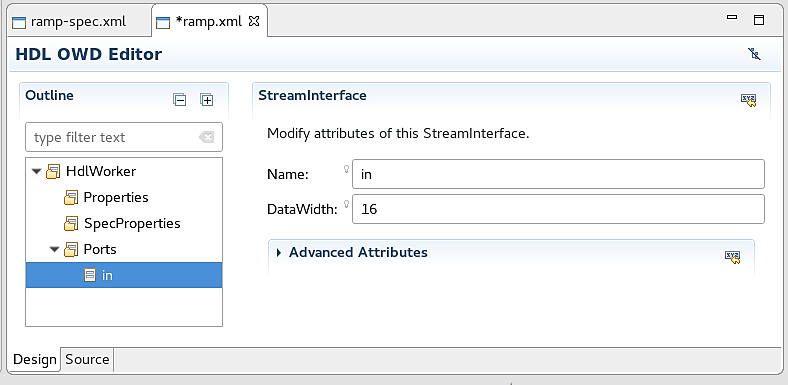
\includegraphics[width=.65\textwidth]{Additionofinandoutinterfaces.png}
 \end{figure}
\subsection{Creating Applications and Assemblies}
The AV IDE Application and Assembly Editors provides a drag-and-drop interface to generate the respective XML files. As an example, the Application Editor is used to create the DemoApp application described in the Getting Started Guide.To start creating, use the Asset Wizard to create a new application:\\
\begin{figure}[h!]
	\centering
	\caption{Asset Wizard New Application}{}
	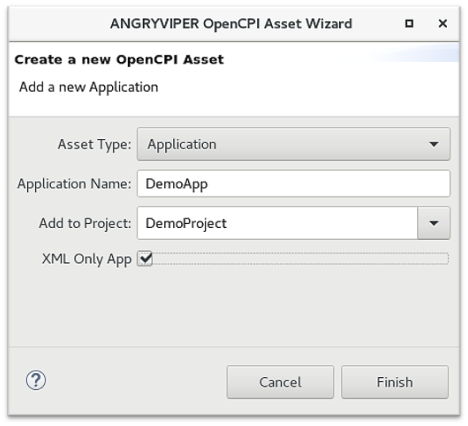
\includegraphics[width=.65\textwidth]{Application_Asset.png}
 \end{figure}

Click Finish and the Application Editor opens:
\begin{figure}[h!]
	\centering
	\caption{Application Editor}{}
	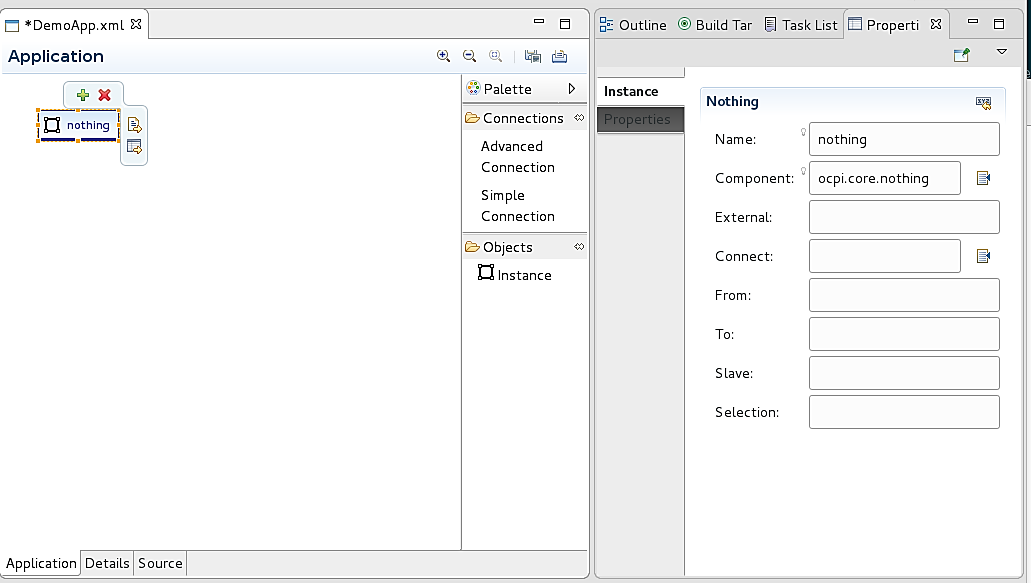
\includegraphics[width=.65\textwidth]{ApplicationEditor.png}
 \end{figure}

\subsection{Adding Components to an Application}
Applications are constructed using OpenCPI Component Specifications (OCS) referred to as components. When the Editor opens, the \textbf{Application Tab} is presented with the \textbf{nothing} instance in the panel.\\
To select a OCS for this instance, click the \textbf{\emph{nothing}} instance and more controls appear. \\

\begin{figure}[h!]
	\centering
	\caption{Properties View}{}
	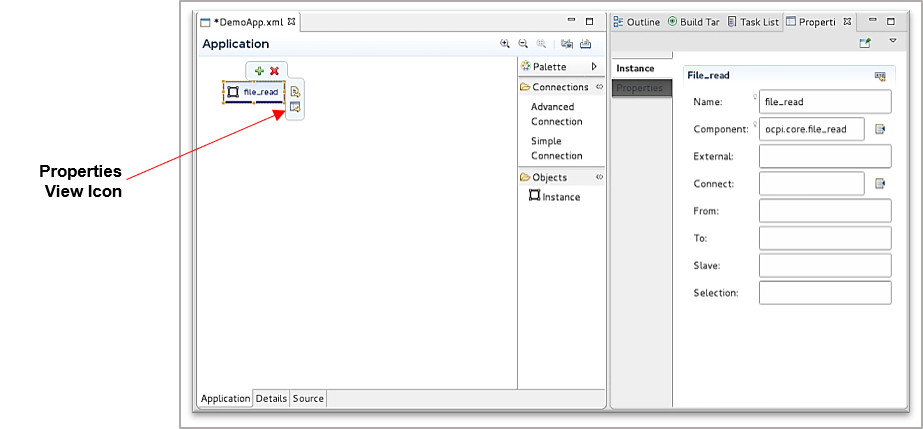
\includegraphics[width=\textwidth]{PropertiesView.png}
 \end{figure}
\bigskip
Select the bottom right icon to see the Properties View Form to further populate the instance. To find the desired OCS, go to the Properties View and click on the List icon next to the component textbox.\\

A listing of all component specifications found in the environment is displayed. The \textbf{ocpi.core.file\_read} component was selected and now the display appears as shown above.\\

The next example adds the local DemoProject.ramp component to the application using drag-and-drop:
\begin{itemize}
\item	Use the Eclipse Project Explorer to Select a component OCS XML file
\item	Left click/hold and drag the file to the Application Panel
\item	Release the mouse button
\item[] As shown below, the ramp component is now in the application. Another method to do this is:
\item	Drag-and-drop the instance object from the Palette into the application panel
\item	Select the component via the Properties View as demonstrated in the example above.
\end{itemize}
\begin{figure}[h!]
	\centering
	\caption{Adding the Ramp Component}{}
	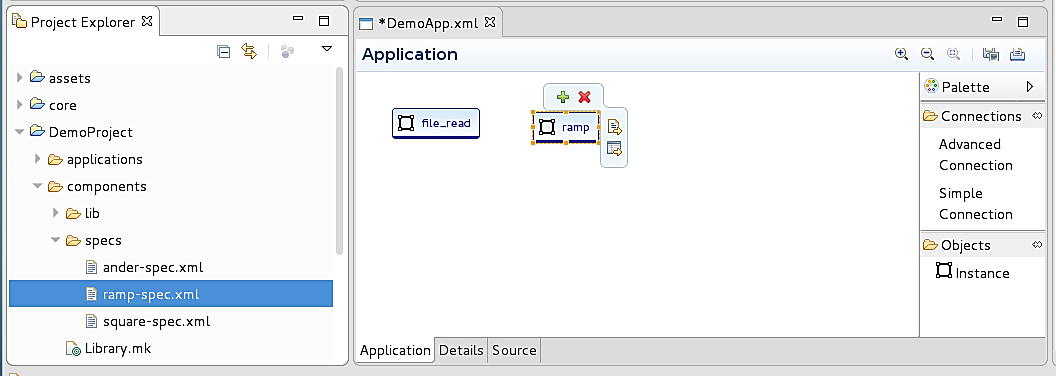
\includegraphics[width=.95\textwidth]{AddingtheRampComponent.png}
 \end{figure}

The third method to construct an application is to use the Details Tab. This tab presents a form-based editor similar to the component and worker editors described above. The Application Details panel is shown in the figure below:\\

\begin{itemize}
\item	Select the Instances element
\item	Click Add an Instance
\end{itemize}
\begin{figure}[h!]
	\centering
	\caption{Third Method to Add a Component Instance}{}
	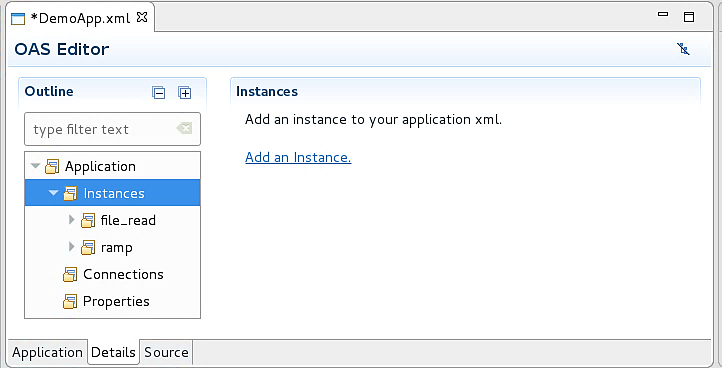
\includegraphics[width=.95\textwidth]{ThirdMethodtoAddaComponentInstance.png}
 \end{figure}
A form opens to populate the new instance as shown in the below image. Note that component choices originate from the current project and its project dependencies.\\
\begin{figure}[h!]
	\centering
	\caption{Select File Write as the New Companion}{}
	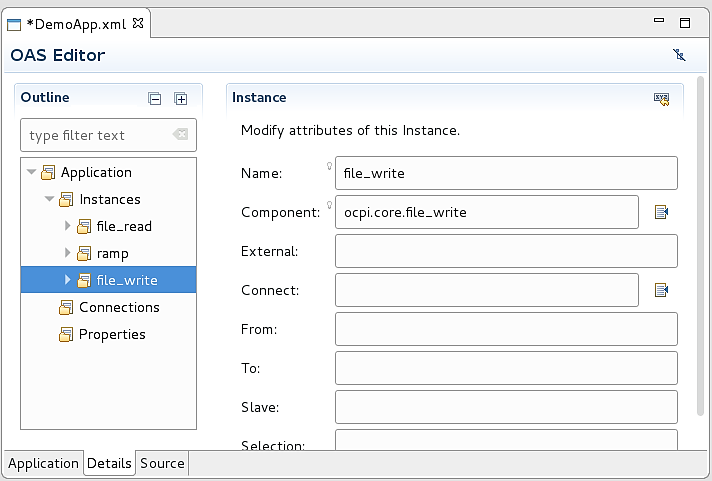
\includegraphics[width=.95\textwidth]{SelectFileWriteastheNewCompanion.png}
 \end{figure}

Click the List icon next to the Component text box input to the components list. The file write component was selected. The below figure shows the current design view of the application.
\begin{figure}[h!]
	\centering
	\caption{Design View of the Application}{}
	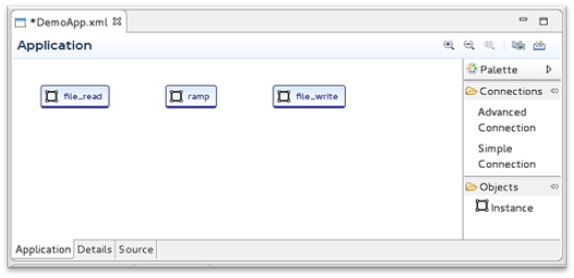
\includegraphics[width=.85\textwidth]{DesignView.png}
 \end{figure}
\subsection{Connecting Application Components}
The Application Editor provides three different methods to create connections between components. If simple connections are sufficient (single in/out components), the simpliest method is to use the application diagram (Application tab) and use the Simple Connection in the palette:
\begin{itemize}
\item Select simple connection in the palette
\item Move the cursor to the source component
\item Click while on it and then move the cursor to the receiving component, click it to complete a connection
\end{itemize}
Complex connection can be added using the palette and is the easiest way as well. \\

The second method is to use the XML node approach accessed using the Details tab:
\begin{itemize}
\item	Simple connections are added by selecting the instance then filling in the "Connect" input (this indicates the component receiving the output of this instance)
\item	Complex connection are not as graceful to accomplish using this method, Click the Connections node in the outline
\item	Click the Add a Connection link
\item	Click add Port, Provide the Port name and instance, it connects as shown in the Advanced Connection Figure below.
\end{itemize}
The third method is to edit the XML source directly. Once the template of a complex connection is put in place, this is likely the easiest method to add complex connections. It is also a good method used to make corrections to the diagram, particularly if instances are removed from the diagram or the component of an instance is changed.

The following figures demonstrate a simple connection:\\
\begin{figure}[h!]
	\centering
	\caption{Connection Example}{}
	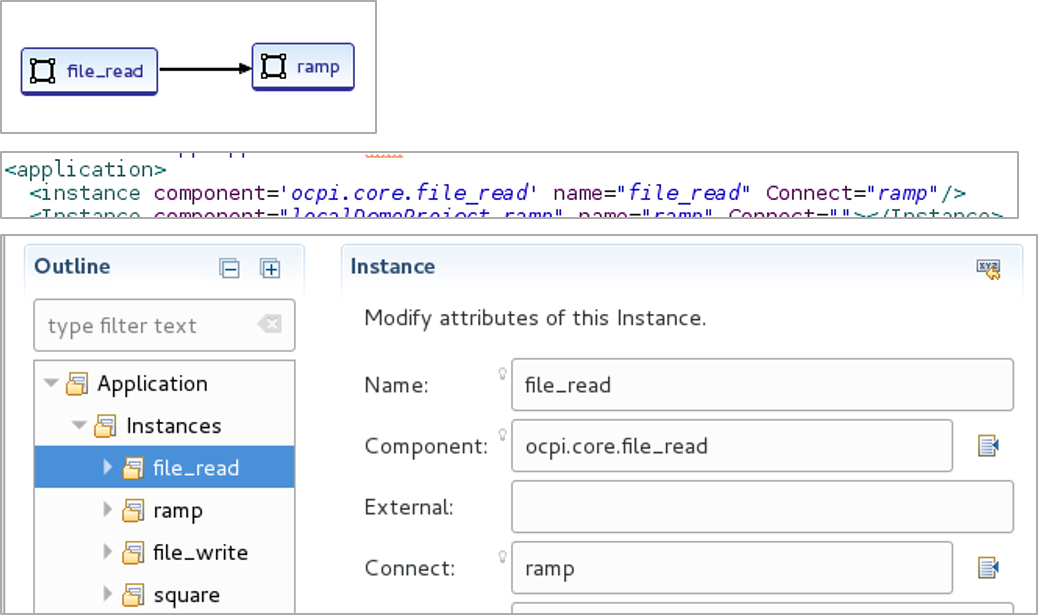
\includegraphics[width=\textwidth]{ConnectionExample.png}
 \end{figure}
Advanced connections are easily created using the Application Tab. To make an advanced connection while in the Application Tab:
\begin{itemize}
\item	Select Advanced Connection in the palette
\item	Move the cursor to the source component
\item	Click it, move the cursor to the destination component and click it again
\end{itemize}
A pop-up form panel appears with inputs to complete the connection as shown below.
\begin{figure}[h!]
	\centering
	\caption{Pop Up Panel}{}
	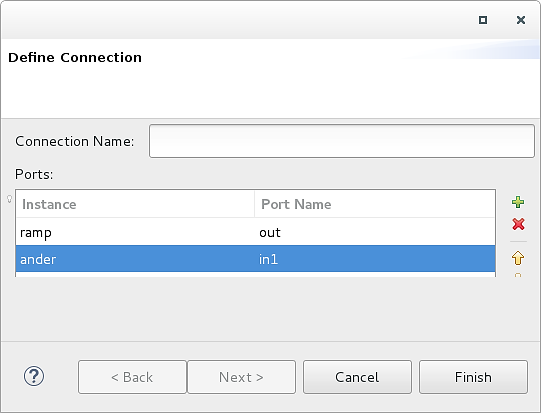
\includegraphics[width=.65\textwidth]{PopUpPanel.png}
 \end{figure}
Advanced connections can be named (optional). The Ports section opens with default Port names \textbf{out and in}. Click on the In-Port name and update it to the correct Port (in1) as shown above.\\

The following series of figures show the advanced connection in the 3 editor views:
\begin{figure}[h!]
	\centering
	\caption{Advanced Connection Views}{}
	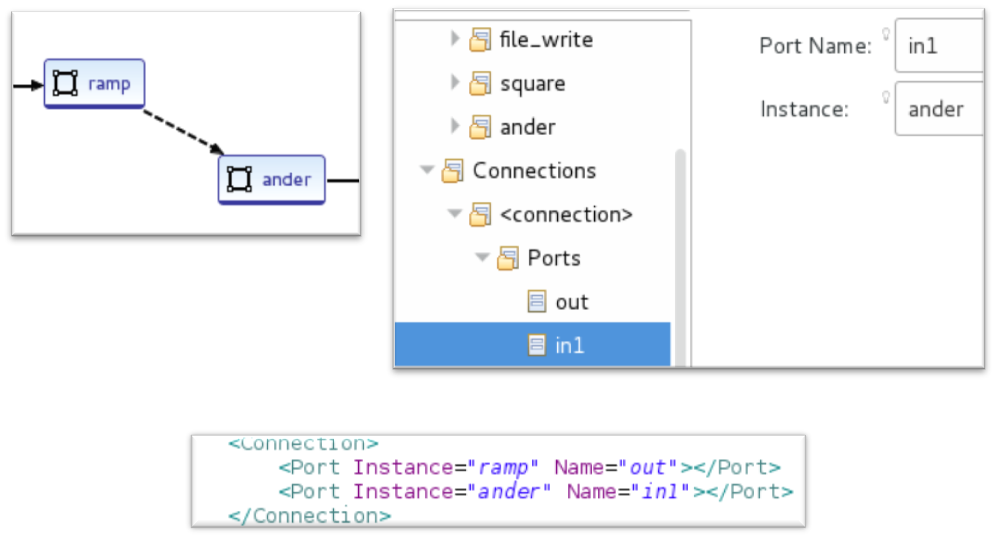
\includegraphics[width=.85\textwidth]{AdvancedConnectionViews.png}
 \end{figure}

See the \githubio[Application Development Guide]{OpenCPI\_Application\_Development.pdf} for detailed information about the Application and Assembly XML files.
Note that the Application and Assembly Editors provide a basic capability to create the respective XML files.
\subsection{Assembly Editor}
The HDL Assembly Editor operates similarly to the Application Editor. The difference is that assemblies are built with application workers while applications are built with components. The drag-and-drop feature works with OpenCPI Worker Description (OWD) XML files just as the application Editor operates with OCS XML files. \textbf{\emph{Note: The Eclipse Project Explorer must be used for the current drag and drop feature; it is currently not supported in the OpenCPI Projects View.}}\\
Below shows the square.hdl worker added to an assembly via drag-and-drop. Also note that worker choices originate from registered OpenCPI projects.
\begin{figure}[h!]
	\centering
	\caption{Square HDL Worker}{}
	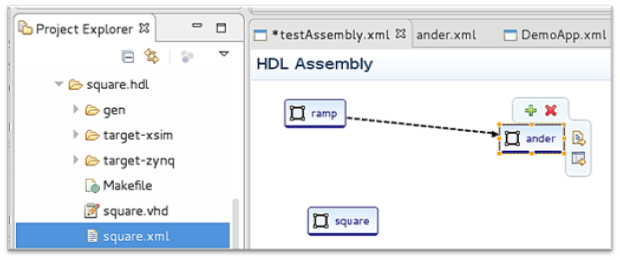
\includegraphics[width=.75\textwidth]{SquareHDLWorker.png}
 \end{figure}
\subsection{Creating Component Unit Tests}
Creating a Unit Test using the Asset Wizard is demonstrated in this section.
\begin{itemize}
\item	Using the OpenCPI Projects View
\item	Navigate to DemoProject
\item	Components
\item	Specs
\item	Select Ramp-Spec.XML
\item	Right-click and select \textbf{New Unit Test} from the context menu.
\item The Asset Wizard opens with all inputs preset for the ramp-spec selection as shown below and then Click Finish.
\end{itemize}
\begin{figure}[h!]
	\centering
	\caption{All Inputs are preset for the Ramp Spec}{}
	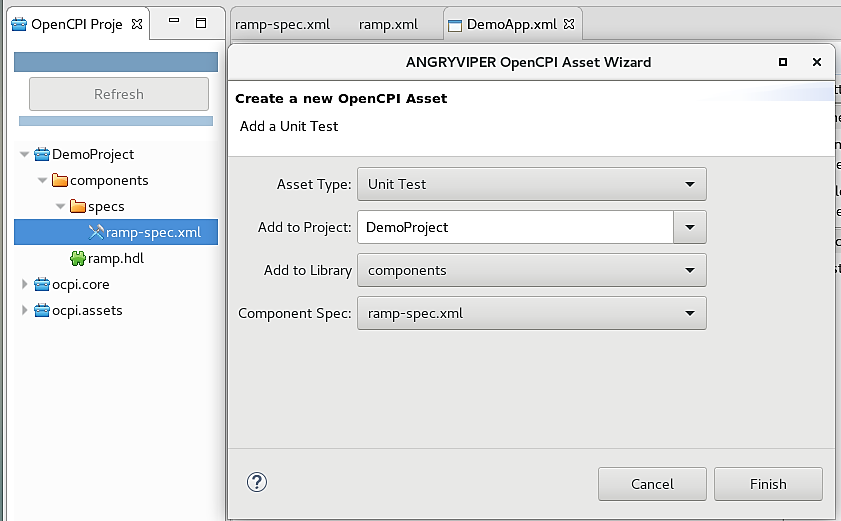
\includegraphics[width=.65\textwidth]{InputsarePresetfortheRampSpec.png}
 \end{figure}
When the action completes, the Unit Test Editor opens in the Editor panel as shown below. \\

Unit testing requires an in-depth knowledge on how to implement them so this will not be addressed here. Refer to the \githubio[Component Development Guide]{OpenCPI\_Component\_Development.pdf} to learn about them.
The Editor supports most aspects of developing unit test XML.\\

\begin{figure}[h!]
	\centering
	\caption{Unit Test Editor Panel}{}
	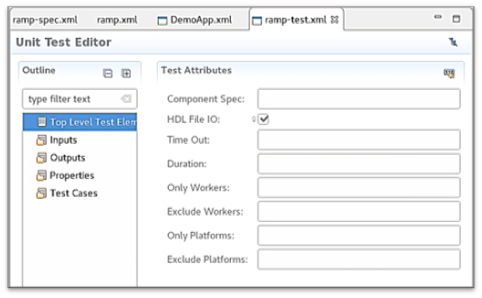
\includegraphics[width=.65\textwidth]{UnitTestEditorPanel.png}
 \end{figure}

\textbf{\emph{Note: There are a number of cases where one attribute out of a set may go in the test XML element. This is very prevalent for the input, output, and test case elements. In this implementation of the Editor, once an attribute out of the set is added, the inputs for other choices are disabled.}}\\

The figure below demonstrates this behavior. An input element can either have a name or a Port and the source data from them can either be a script or a file, so once filled in the other inputs are disabled. Simply clear the input to start over (use backspace or select delete).\\
\begin{figure}[h!]
	\centering
	\caption{Display of Attribute Choice}{}
	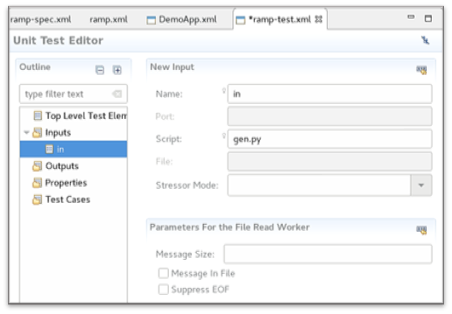
\includegraphics[width=.65\textwidth]{DisplayofAttributeChoice.png}
 \end{figure}


\newpage
\section{Appendix A}
\subsection{Eclipse Basics}
A central abstraction for Eclipse is \textbf{the workspace}. This is a directory Eclipse uses to maintain state and projects. When Eclipse opens, it prompts the user to Select a workspace with the following dialog preset for a default directory name in the user’s home directory. If the workspace directory does not exist yet, it will be created. This directory path name can be changed. The Browse Button allows navigation to another location to either create the workspace or select an existing workspace directory.
 \begin{figure}[h!]
	\centering
	\caption{Eclipse Launcher}{}
	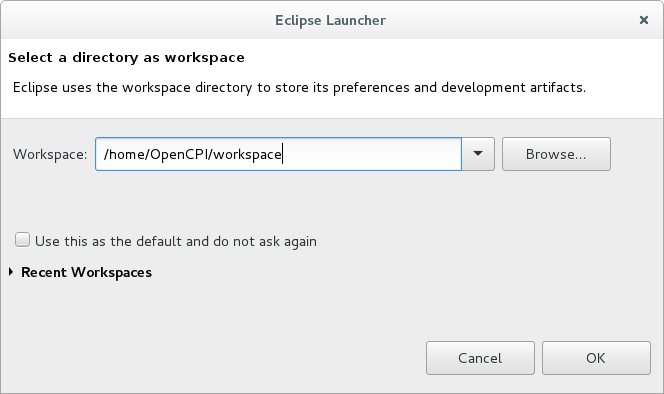
\includegraphics[width=.70\textwidth]{EclipseLauncher.png}
 \end{figure}

Since this is a new workspace, when Eclipse completes start-up, it presents the Welcome screen as shown in the figure below. If you are new to Eclipse or an IDE of this type, this is a good screen to explore. Overview gives basic concepts and definitions such as Toolbars, Perspectives, and Views.
\begin{figure}[h!]
	\centering
	\caption{Eclipse Welcome Screen}{}
	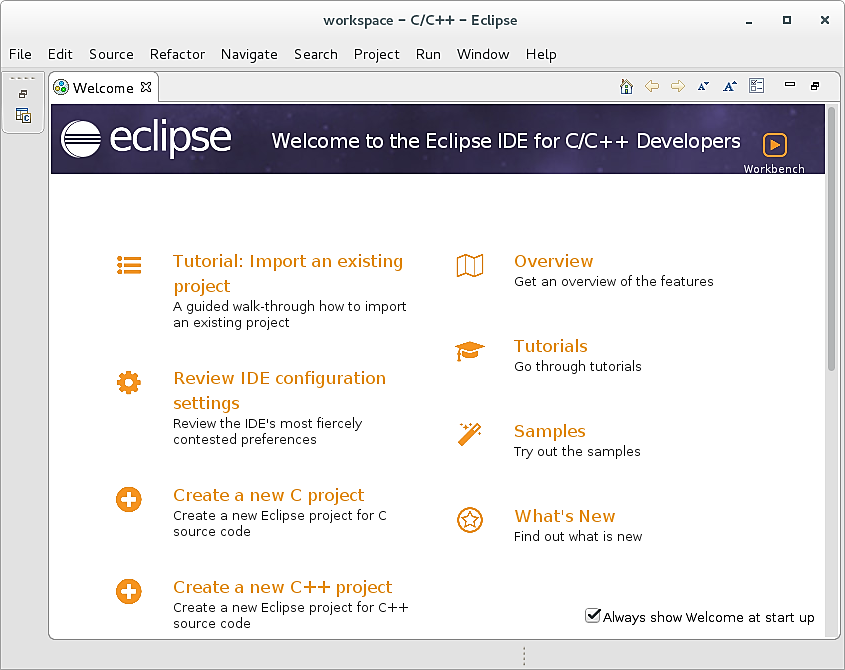
\includegraphics[width=.70\textwidth]{EclipseWelcomeScreen.png}
 \end{figure}
The other selections provide how-to instruction. To continue to see this screen when Eclipse opens, keep the "Always Show Welcome on Startup" check box checked and go through these items. \\

For now, move on to the workbench:
\begin{itemize}
\item Click the workbench arrow button in the upper right corner
\item When the workbench first opens, the IDE defaults to the C/C++ perspective1 as show in figure below
\end{itemize}
 {\textbf {Note: Section 3 above explains how to open the Perspective and how to use the IDE for OpenCPI development is explained in Section 5.}}\\

\emph{Note: Even if Eclipse projects are placed in the workspace directory, Eclipse will not bring them into the workspace. Projects must be imported or locally created to be appear in the Project Explorer View.}\\

OpenCPI projects will not appear in the OpenCPI Projects View unless they are open projects.\\

\begin{figure}[h!]
	\centering
	\caption{Eclipse Workspace}{}
	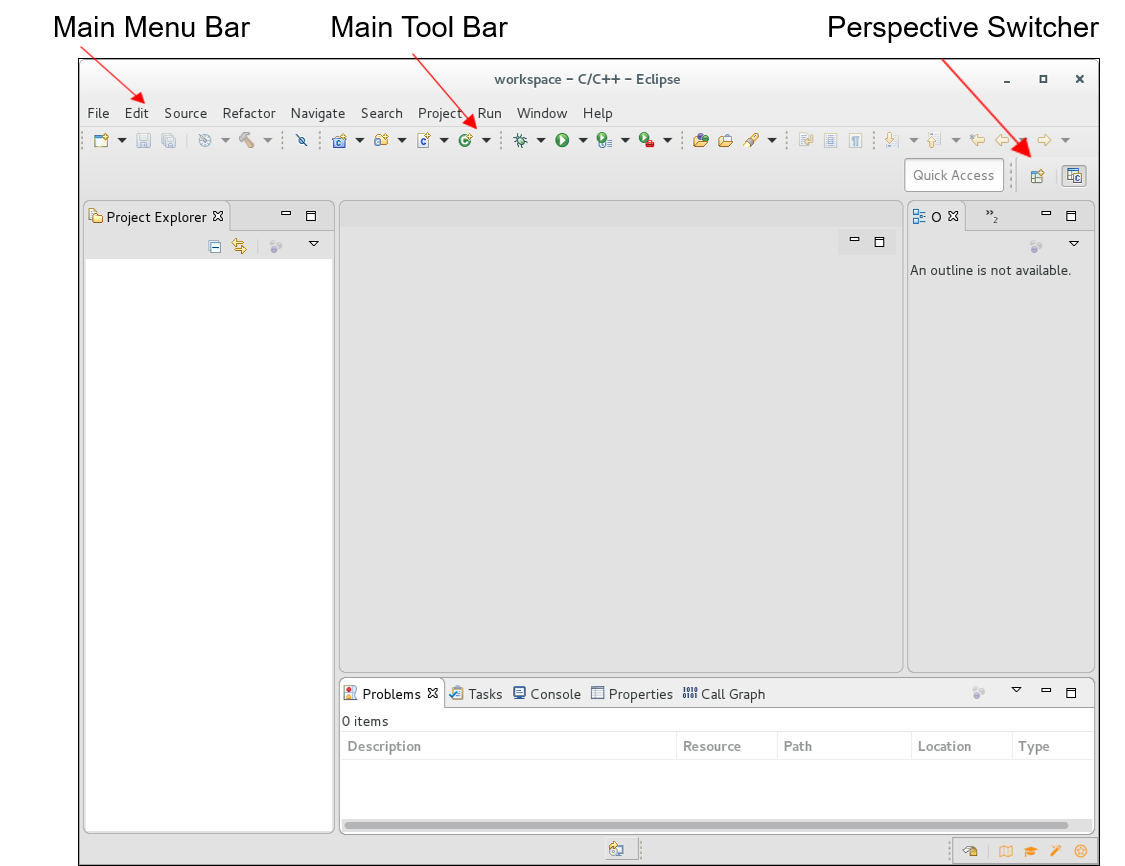
\includegraphics[width=\textwidth]{EclipseWorkspace.png}
 \end{figure}

\section{Eclipse Basic Concepts}
Eclipse uses \textbf{Perspectives} to provide various sets of tools that together focus on a given perspective of development. A perspective consists of a workbench layout of a complimentary set of Eclipse views. A \textbf{view} is a workbench panel that provides a specific capability. For example, the Eclipse Project Explorer View provides a graphical view of the file system and the ability to navigate through and act upon it. The Window Tab in the Main Menu Bar at the top of the window provides navigation to the available perspectives and views, as well as, workbench window controls and user preferences. \\

A final note: the user can rearrange a perspective layout, add, or remove views, and modify panel sizes. These setting are saved and become the default layout for that perspective. Projects must be imported to appear in the workspace. The Eclipse Project Explorer provides these controls via a context menu that is opened by right-click when the cursor is in the view. This menu provides access to create new things in the workspace or project, controls to open or closed a project and to remove files, folders, and projects from the workspace.\\

\textbf{\emph{Caution! Using Project Explorer to delete OpenCPI assets can cause problems; deleting/renaming source files is okay. It is okay to remove a project from the workspace (delete is used), however, do not remove OpenCPI project contents from the file system unless it has been unregistered}}. \\

The OpenCPI Projects View or the ocpidev command should be used to delete OpenCPI projects and assets. Editors and tool chains – Review the Workbench Overview panel and look over C/C++ Development documentation.
\newpage
\section{Appendix B}
\subsection{Additional Plugins for the IDE}
If the development machine has access to the internet or a mirrored Eclipse Marketplace, consider the following software to enhance the AV IDE experience. The Marketplace link is found under the Help link in the top navigation bar. The Marketplace makes it very easy to search, browse and review software. Using the IDE navigate to Help-Eclipse Marketplace. Search for the packages below; it is a simple install button click to get the package.\\
\subsection{TM Terminal 4.0}
Search for Terminal in the Marketplace to see a number of available terminal packages. The TM Terminal 4 has been used successfully by the AV team. Click the install button to install the product. Typically, an agreement must be excepted to continue.\\
\end{document}
